\documentclass[journal]{IEEEtran}
\pagenumbering{arabic}
\usepackage{graphicx}
\usepackage{epsfig}
\usepackage{psfrag}
\ifCLASSOPTIONcompsoc
   \usepackage[caption=false,font=normalsize,labelfont=sf,textfont=sf]{subfig}
\else
   \usepackage[caption=false,font=footnotesize]{subfig}
\fi

\begin{document}
% paper title
\title{Decentralized Frame Synchronization of a TDMA-based Wireless Sensor Network}
% author names and affiliations
% use a multiple column layout for up to three different
% affiliations
\author{\IEEEauthorblockN{}
\IEEEauthorblockA{Fasika Assegei\\ Radiocommunication Group\\
Department of Electrical Engineering\\
Eindhoven University of Technology\\
Eindhoven, The Netherlands\\
Email: f.a.assegei@student.tue.nl}}

\markboth{M.Sc. Graduation Paper F.A.Assegei - Department of Electrical Engineering, TU/e}
{Decentralized Frame Synchronization of a Wireless Sensor Network}

\maketitle

\begin{abstract}
Synchronization is a crucial component of infrastructure for
\textit{Wireless Sensor Networks}(WSNs). Most applications of WSNs
make extensive use of synchronization mechanisms like  \emph{Time
Division Multiple Access} (TDMA) scheduling, accurate timestamping
of events, coordinate activities of the network or data fusion. The
unique requirements of WSNs in terms of precision, lifetime, energy
and scope of the synchronization achieved make the traditional
synchronization methods unsuitable for WSNs. This motivates the
research of synchronization methods which are aligned to the
specific challenges posed on WSN synchronization. \newline In this
research, three algorithms have been developed to achieve a
decentralized, fault-tolerant and energy-efficient synchronization
of a TDMA-based WSN. The algorithms achieve synchronization by using
the phase error of a node's wake-up time with that of the
neighboring node's, without actually exchanging the information
about the clock time of the sender. So, the methods avoid time
keeping on the messages(time stamping) which reduces the message
overload. The algorithm can be integrated with the slot allocation
algorithm  for a better throughput. The research is concluded with
the comparison of these algorithms in terms of energy consumption
and performance.
\end{abstract}
\begin{IEEEkeywords}
adhoc networks, frame synchronization, decentralized synchronization, wireless sensor networks.
\end{IEEEkeywords}
\section{\textbf{Introduction}}
\subsection{\textbf{Synchronization in Wireless Sensor Networks}}
\noindent WSNs are distributed networks of low cost sensors, dedicated to closely observing real-world phenomena.
 Various applications are realized using WSNs$\cite{10}$. One of the design issues in WSN technology is synchronization, which is a critical piece of infrastructure in any distributed system. There are many reasons why a synchronized time is needed in a WSN, one of them being adjusting the slots in a TDMA-based communication. \newline
In order to have a seamless communication between the nodes, the synchronization of the frames is a necessary part of the MAC
protocol. Due to physical factors, the frequency of the oscillator in the node has a drift. When no provisions are taken, it causes the nodes to run out of synchronization. Given that there is a certain error, the node will adjust its wake-up time with the offset calculated with a synchronization algorithm.
\subsection{\textbf{Existing Work on WSN frame synchronization}}
\noindent Several algorithms have been proposed and researched for
frame synchronization in WSNs. The \textit{Reference Broadcast
Synchronization} (RBS) stated in $\cite{2}$ is an important scheme
in the area of WSN synchronization. It achieves a Receiver-Receiver
pairwise synchronization to remove sender nondeterminism and results
in a good precision of a few microseconds. A decentralized slot
synchronization algorithm  for TDMA-based networks is shown in
$\cite{3}$. This method uses the topology of the nodes as a means to
weigh the phase error of the sender with the receiver. \newline
Another approach stated in $\cite{texas}$ establishes a table to
correspond the clock of the sender with that of the receiver clock
so that a good estimation of the neighbors clock is achieved using
different estimation techniques. A different approach to
weight-based synchronization for interference elimination for a TDMA
based ad-hoc networks is presented in $\cite{6}$. The algorithm
achieves synchronization in a decentralized manner using the node's
phase error with its neighbors' to eliminate the impact of
interference. Correlation method is used in $\cite{correlation}$
inorder to decode the message and learn about the status of the
sender node which is used for synchronization.
\subsection{\textbf{Objective and overview of the research}}\noindent
The primary objective of this research is to develop an algorithm to
achieve a long-term decentralized frame synchronization of a WSN in
an energy-efficient method which employs no timestamping on the
messages. The method use the phase errors between the receiver and
its neighbors, without actually estimating the neighbor's clock as a
way of achieving long-term frame synchronization. In this research,
three algorithms are presented to achieve a long term decentralized
synchronization of a WSN and compared in terms of performance and
energy consumption.
\newline The remainder of the paper is organized as follows:
Section 2 discusses the synchronization error and formulate the problem.
Section 3 presents the mathematical models of the algorithms for the synchronization of the network.
 In Section 4, simulation results are presented and analysis of the results in addition to the comparison of the methods with respect to energy consumption is discussed.
Finally, Section 5 draws the conclusions from the research and suggests future work.
\section{\textbf{Problem Formulation}}
\subsection{\textbf{Wireless Sensor Networks: Why different ?}}
\noindent Are traditional synchronization methods applicable in the case of WSNs? Many
assumptions in the traditional schemes do not hold in the case
of WSNs. Some of these factors can be described as follows:
\begin{itemize}
\item \textbf{Energy Limitation}: Due to the nodes' small size and nature of applications which they
are designed for, energy consumption is a major concern in a WSN.
\item \textbf{Dynamic Nature of the Network}: In a WSN, network
dynamics results from various factors which prevents simple
static configurations.
\item \textbf{Diverse Applications}: A variety of applications
have totally different needs as far as synchronization is concerned.
Some applications might need a global timescale while
others can work with a relative timescale.
\item \textbf{Cost of the Nodes}: Sensor nodes are very small in size
and must be cheap cost wise.
\end{itemize}
\subsection{\textbf{Sources of synchronization error}}\noindent
The different factors which give rise to errors between two nodes can be identified as:\newline
\textbf{Oscillator Characteristics}: The following two oscillator characteristics are the main sources of errors between the clocks of two different nodes.
         \begin{itemize}
         \item \emph{\textbf{Accuracy}}: is a measure of the difference between oscillators expected (ideal)
           frequency and actual frequency.
         \item \emph{\textbf{Stability}}: is oscillator's tendency to stay at the same frequency over
           time.
      \end{itemize}
\textbf{Hardware and Environmental factors}: The non-determinism in the message delivery latency can be categorized in four type of delays:
      \begin{itemize}
         \item \emph{\textbf{Send Time}}: The time spent at the Sender to build the message.
         \item \emph{\textbf{Access Time}}: Delay occurred while waiting for access to the transmit channel.
         \item \emph{\textbf{Propagation Time}}: Time required for the message to travel from sender to receiver.
         \item \emph{\textbf{Receive Time}}: Time needed for processing at the receivers.
      \end{itemize}
All the above factors result in following errors between two nodes:
\begin{itemize}
\item \textbf{Phase error}: The oscillators of any two nodes can be out of phase at any given time, resulting into different time on both clocks.
\item \textbf{Frequency error}: Frequency error, in contrast, measures the difference in the clock rates.
\item \textbf{Clock drift}: It is not just that the clocks are running at different rates, but the frequency of each clock does not stay constant over a period of time.
\end{itemize}
\subsection{\textbf{Clock Time}}
%\begin{figure}[b]
%\centering
%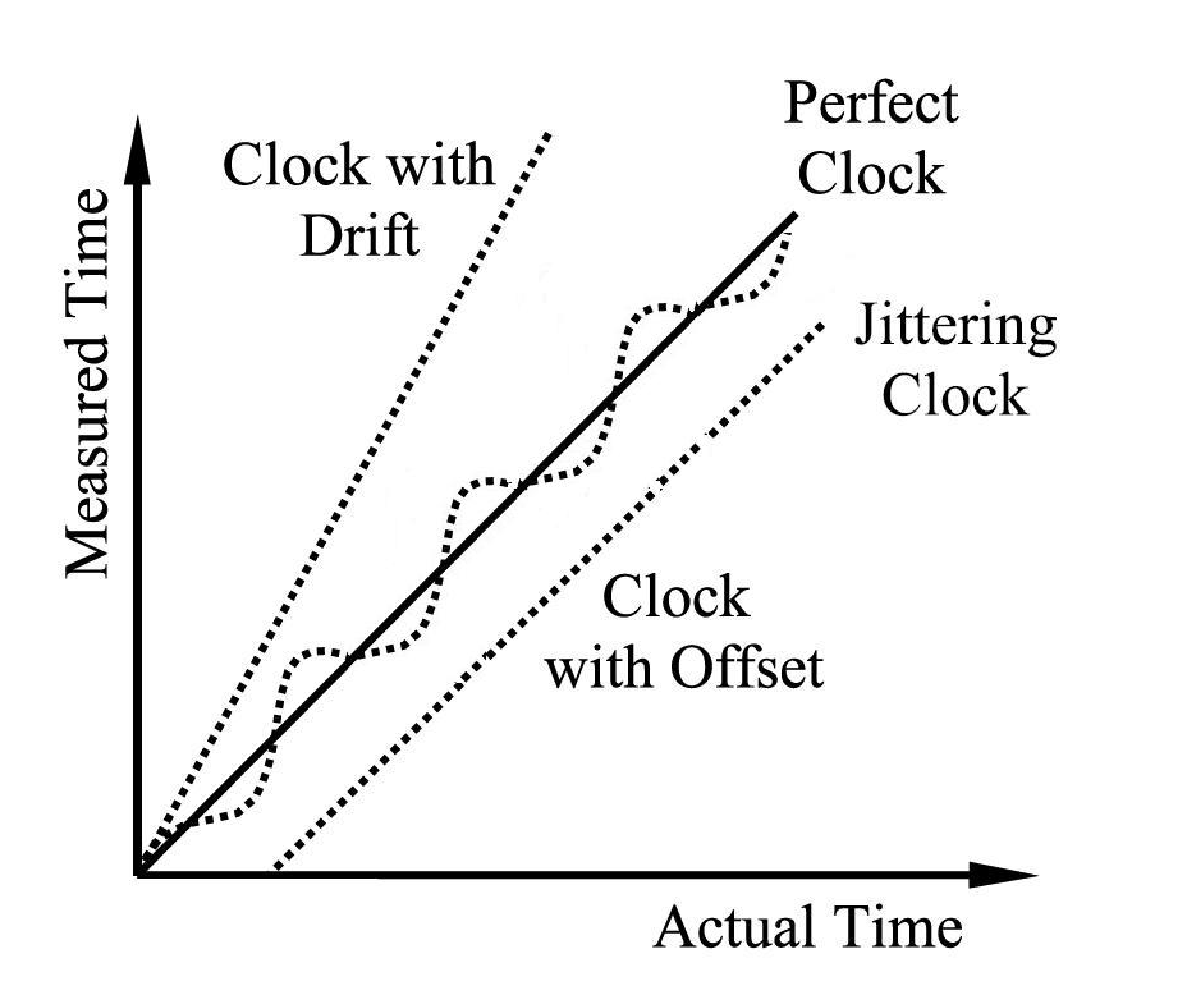
\includegraphics[width=0.35\textwidth]{actualvsmeasuredtime}
%\caption{Measured time versus real time}
%\label{fig:clocktimevsrealtime}
%\end{figure}
\noindent From the definition of frequency:
\begin{equation}
f = d\phi/dt \label{freq_defn} ,
\end{equation}
and integrating both sides over time,
 \begin{equation}
\phi =\int f(t)dt ,
 \end{equation}
where $f$ is frequency, $\phi$ is phase, and $t$ is time.\newline
Thus, the clock time is described as
\begin{equation}
C(t) = \frac{1}{f_o}\int_{t_o}^{t} {f(\tau)d\tau} + C(t_o) ,
\label{clock}
\end{equation}
where $f(\tau)$ is the frequency of the clock, $f_o$ is the nominal frequency of the crystal oscillator and $t_o$ is the start time of the node. \newline The exact clock drift is hard to predict because it depends on environmental influences but can usually assumed that it clock doesn't exceed a maximum value $\rho$. This means that it can be assumed
\begin{equation}
1-\rho \leq \frac{dC(t)}{dt} \leq 1+\rho ,
\end{equation}
where $\rho$ represents the maximum clock drift. Note that different clocks have different maximum clock drift values $\rho$.\newline The frequency of the clock is dependent on different
factors and can be given as
\begin{equation}
f_i(t) = f_o + \Delta f + a(t-t_o) + \Delta
f_e(t-t_o) + f_r(t) \label{frequency}
\end{equation}
where \newline $t_o$ = the start time of the clock, \newline $a$ = aging factor,  \newline $f_o$ = nominal frequency, \newline $\Delta
f$ = calibration error,\newline $f_r(t)$ = frequency instability (noise) term, \newline $\Delta f_e$ = frequency error which occurs
due to outside factors like temperature, voltage instability. \newline
From ($\ref{clock}$) and ($\ref{frequency}$),
\begin{equation}
C_i(t) - C_i(t_o) = \frac{1}{f_o} \int^{t}_{t_o}f_i(\tau)d\tau ,
\end{equation}
\begin{eqnarray*}
C_i(t) - C_i(t_o) & = & \frac{1}{f_o} \int^{t}_{t_o}{[f_o + \Delta f + a(\tau-t_o)  } \\
 &  & {} + \Delta f_e(\tau-t_o) + f_r(\tau)]d\tau ,
\label{fasika}
\end{eqnarray*}
\begin{eqnarray*}
C_i(t) & = & C_i(t_o) + (t-t_o) +\frac{\Delta f}{f_o}(t-t_o) \\
& & + \frac{a}{2f_o}(t-t_o)^2 + \frac{\Delta f_e}{2f_o}(t-t_o)^2 +
\frac{1}{f_o}\int^{t}_{t_o}{f_r(\tau)d\tau} .
\end{eqnarray*}
\subsection{\textbf{Median algorithm and the setback}}
The Median algorithm is currently implemented in the MyriaNode.
The algorithm is described as follows:
\begin{enumerate}
\item Nodes broadcast packets.
\item Each receiver records the time that the packet is received according to the local clock.
\item Each receiver $i$ computes its phase errpr to
any other node j in the neighborhood as
\begin{equation}
\Delta t_{ij}^{(n)} = t_i^{(n)} - t_j^{(n)} ,
\end{equation}
where $t_i$ is the wake-up time of node $i$ and $t_j$ is the wake-up
time of node $j$ at the $n^{th}$ period.
\item Receivers compute the median of the offsets
\begin{equation}
\xi_i^{(n)} = median(\Delta t_{ij}^{(n)}) , \forall j
\end{equation}
\item Receivers adjust their wake-up time by the computed offset value,
\begin{equation}
t_{i}^{(n+1)} = t_i^{(n)} + T_i^{(n)} - k\xi_i^{(n)},
\end{equation}
where $k$ is the gain factor.
\end{enumerate}
\begin{figure}[b]
\centering
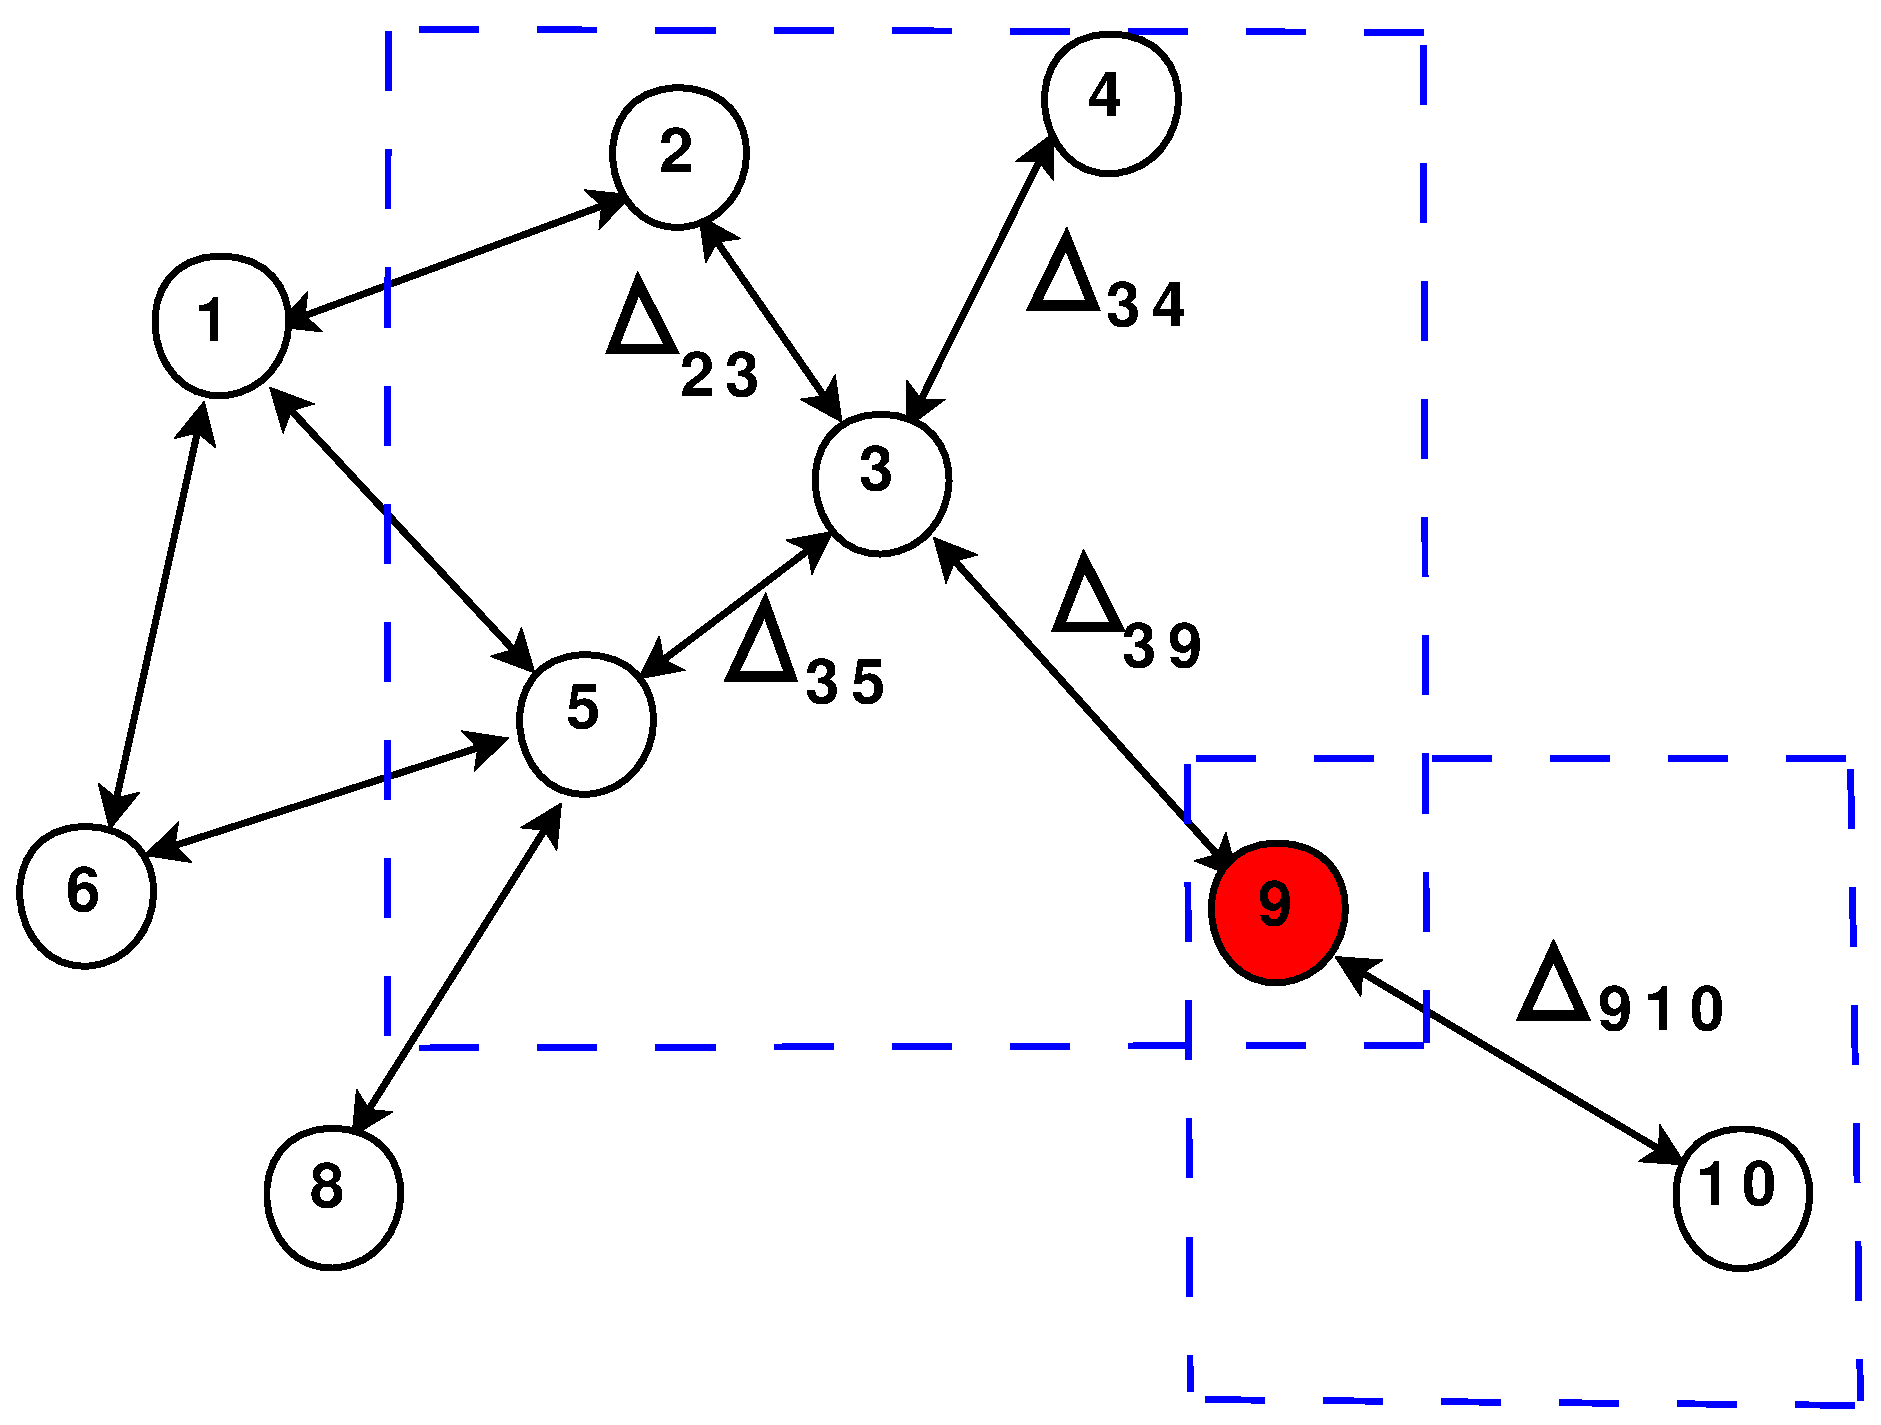
\includegraphics[width=2.5in]{node_field}
\caption{A WSN scenario} \label{wsn}
\end{figure}
By multiplying the median with a gain factor,
i.e. $k\xi_i^{(n)}$, the output can be adjusted for better
performance.
\newline As per the application of Median, there are setbacks on its implementation. In some test-cases, the algorithm fails to converge or stays unsynchronized for a certain period of time.
\newline A typical scenario is presented where the Median algorithm takes a longer time to achieve synchronization. In Figure $\ref{wsn}$, a distribution of nodes is shown. Node 10 joins  the stable network communication through Node 9. Assume Node 9 belongs to two broadcast domains, Node 3's and Node 10's. Thus, upon the application of the median algorithm, the node tends to adjust its wake-up time with the median of the phase errors from its neighbors, Node 3 and Node 10. Adjusting the wake-up time, the offset is
\begin{equation}
\xi_9 = \frac{\Delta t_{910} + \Delta t_{39}}{2}.
\end{equation}
\begin{figure}[t]
\centering
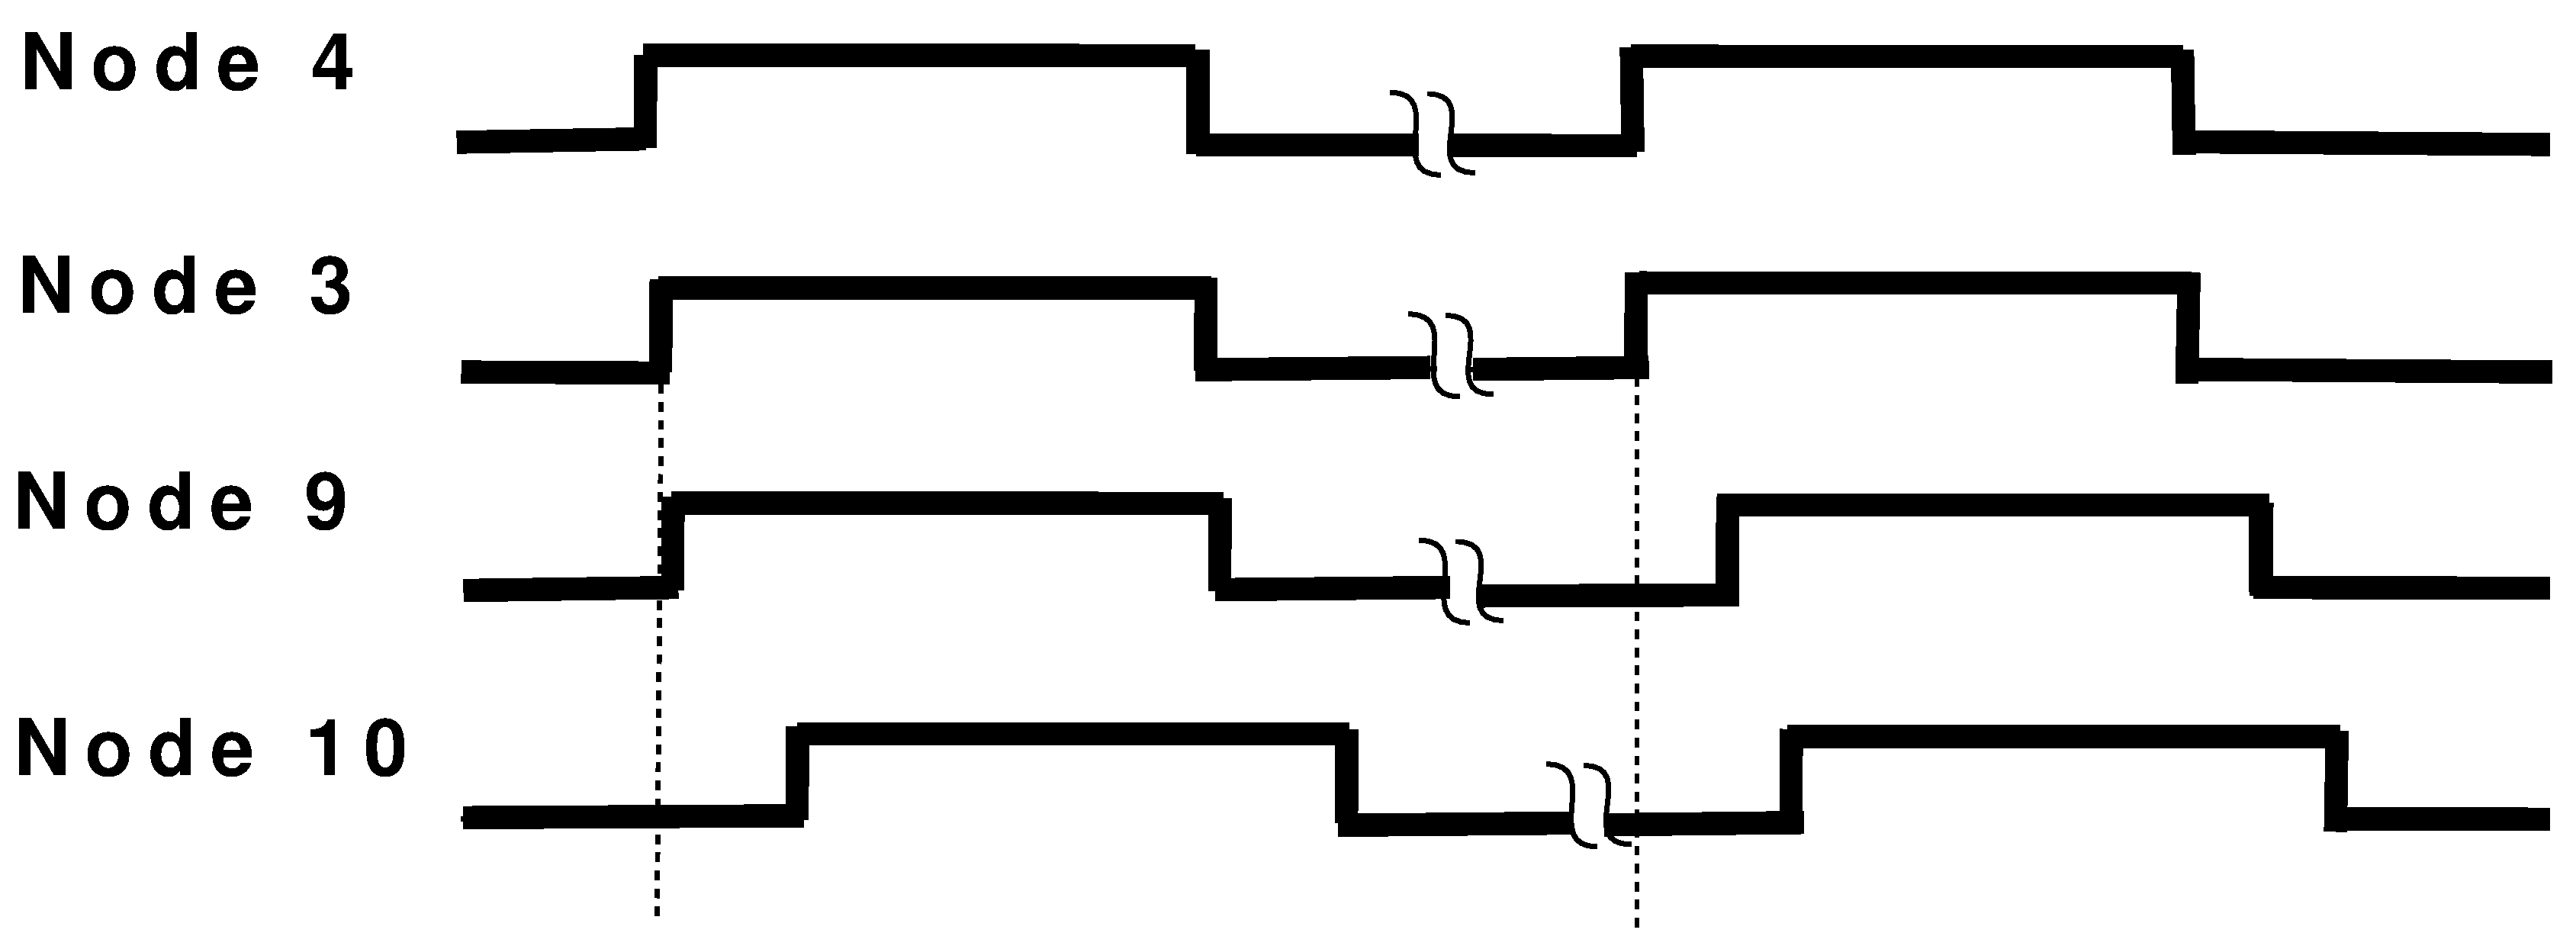
\includegraphics[width= 2.5in]{offsetpic}
\caption{Using median for phase error correction} \label{fasik}
\end{figure}
\noindent With Node 10 being isolated from the well established
network, it has a major drift from the other nodes. Being in sync
with the other nodes, Node 9 will drift away from the network after
its adjustment with the Node 10. It will take more time to
synchronize with the network again. Figure $\ref{fasik}$ shows the state of the network after the
synchronization using the Median.
\newline So, in order to address this problem, three algorithms are explored in the next subsections to realize an energy-efficient, more precise and simple frame synchronization.
\section{\textbf{Synchronicity protocol}}
\subsection{\textbf{Synchronization Frequency}}
\noindent \textbf{Precise synchronization}: Precise synchronization is implemented when a node has already joined in the network, which repeatedly adjusts the diversion of its time slot reference caused by propagation delay and clock drift. \newline \noindent
\newline \noindent
Decreasing the timing of the synchronization and do periodic execution of the synchronization of the algorithm greatly reduces
the energy consumption of the WSN. Thus, a synchronization period, $T_{sync}$, is defined as the period in which the network can stay synchronized without the application of the synchronization algorithm.
\begin{figure}
\centering
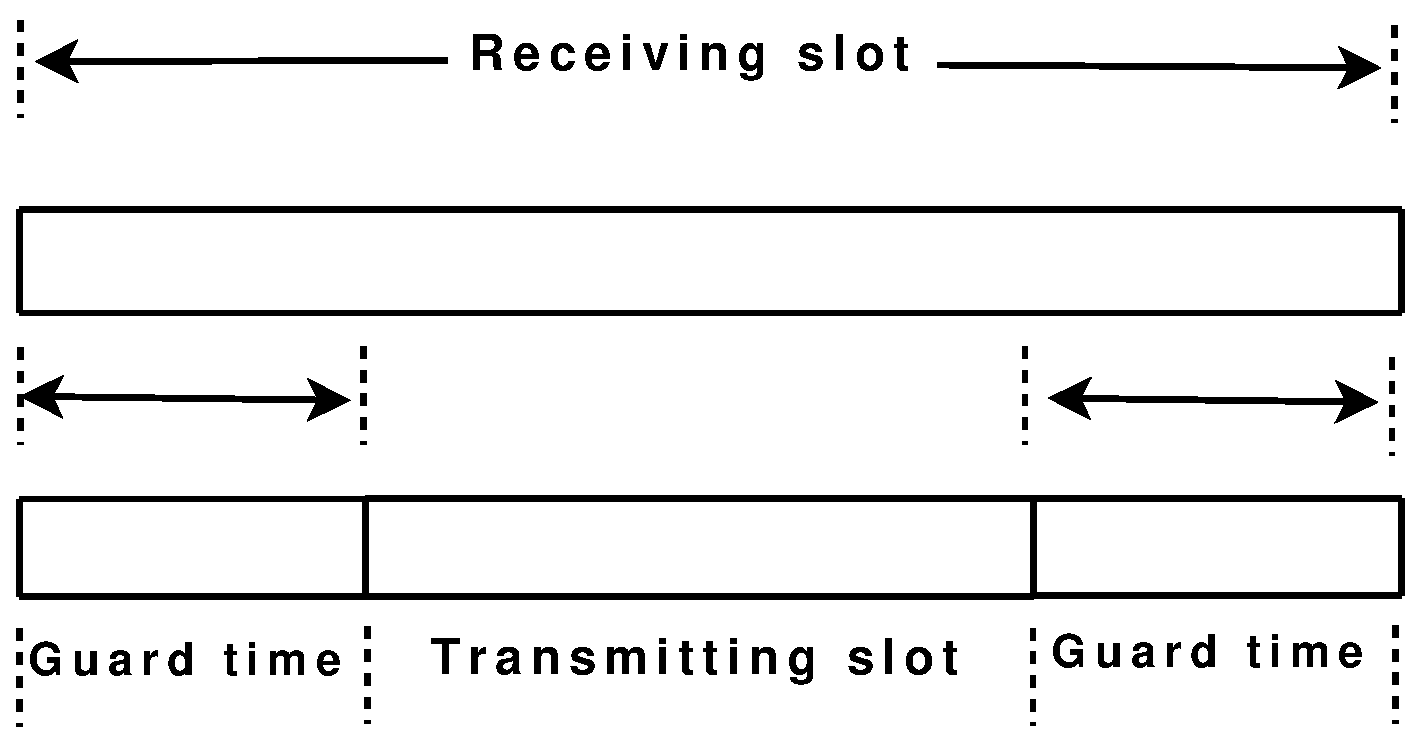
\includegraphics[width=2.5in]{guardtime}
\caption{Guard time of the nodes} \label{guardtime}
\end{figure}
\newline A time slot can be defined as being expressed in a
number of clock cycles as
\begin{equation}
t_{slot} = kT ,
\end{equation} where $T$ is the period of the time frame in clock cycles and
$t_{slot}$ is the time duration of a TDMA slot and $k$ is coefficient.
\newline With a synchronization period $T_{sync}$ and the
maximum clock drift of a clock $\rho$ , the maximum time difference
between a sender and a receiver is
\begin{equation}
t_{diff} = 2\frac{T_{sync}}{T}\rho ,
\end{equation}
where the factor of $2$ reflects the worst case scenario where each
node's clock drifts in the opposite direction.\newline
In achieving frame synchronization in a TDMA scheduling, a guard time is given for a fault tolerance which is used to accommodate the
phase errors, as shown in Figure $\ref{guardtime}$.  Since the
relative time difference between two nodes can be in two direction,
the guard time needs to be twice $t_{diff}$,
\begin{equation}
t_{guard}= 2t_{diff} = 4\frac{T_{sync}}{T}\rho.
\end{equation}
At this end, the minimum duration for a time slot $t_{slot}$ is
\begin{equation}
t_{slot} \geq t_{guard} + T_{tx},
\end{equation}
where $T_{tx}$ is the time required to send a packet from one node to other.
\newline Two nodes have a good communication link when they synchronize
their clocks at least once every $T$ that gives the following
relation,
\begin{equation}
\frac{T_{sync}}{T}\geq 1.
\end{equation}
To obtain the value of $T_{sync}$ for a particular system with a given duty cycle, the following equations are to be seen:
\begin{equation}
t_{guard} \geq 4\rho \frac{T_{sync}}{T}
\end{equation}
\begin{equation}
t_{slot} \geq t_{guard} + T_{tx}
\end{equation}
\begin{equation}
\frac{T_{sync}}{T} \geq 1.
\end{equation}
In general, there is a trade-off in determining $T_{sync}$: increasing $T_{sync}$ reduces the energy costs of synchronization, whereas decreasing the network performance.
\subsection{\textbf{Mathematical Model}}
\noindent As part of the message, nodes are transmitting the slot number which they are transmitting. This information is used in the determination of the time that the message is sent. Each message
that is send within a time slot is exactly received by a neighbor at
a known clock tick number
\begin{equation}
tick_{rx} = T_{tx}+ \frac{t_{guard}}{2} \label{tick}
\end{equation}
Whenever this number is not equal with the desired one, a phase error is observed. \newline
The difference between the wake up times of node $i$ and node $j$ is
\begin{equation}
\Delta t_{ij}^{(n)} = t_i^{(n)} - t_j^{(n)} ,
\end{equation}
where $t_i$ and $t_j$ are the wake-up times of node $i$ and node $j$
at the $n^{th}$ period. \newline \noindent
The wake-up time of a node at a random time after $n$ periods of firings after it is turned on is
\begin{equation}
t_i^{(n)} = \sum_{n} T_i^{(n)} + t_{io},
\end{equation}
where  $T_i^{(n)}$ is the period of the crystal clock at the $n^{th}$ period which changes with time according to ($\ref{frequency}$) and $t_{io}$ is the initial start-up time of the node. The frequency of the node varies due to the different factors mentioned in ($\ref{frequency}$). \newline
The difference in the wake-up time of the nodes is given by
\begin{eqnarray}
\Delta t_{ij} & = & \sum_{n}T_i^{(n)} + t_{io}- (\sum_{n}T_j^{(n)} +
t_{jo}) \\ &=& (\sum_{n}T_i^{(n)} - \sum_{n}T_j^{(n)}) +
(t_{io}-t_{jo}).
\end{eqnarray}
This phase error can be adjusted using two approaches, which are not exclusive. The first
one is adjusting the clock frequency to come up with a better
wake-up time. The second one is to adjust the next wake-up time
depending on the difference between the current wake-up time of the
node and its neighbors. In this research, the second option is
explored due to:
\begin{itemize}
\item The cost of adjusting the frequency of the clock, and
\item The complexity of the implementation.
\end{itemize}
Hence, the next wake-up time of the node is
dependent on the current wake-up time of its neighbors in relation
to its previous wake-up time,
\begin{equation}
t_i^{(n+1)} = t_i^{(n)} + T_i^{(n)} - \xi_i^{(n)} ,
\end{equation}
where $T_i$ is the period of the node's clock and $\xi_i$ is given
by
\begin{equation}
\xi_i = f(\Delta t_{ij}).
\end{equation}
The function $f$ is based on an algorithm which takes the wake-up
time differences between the node and its neighbors and determines
the optimal offset to be added to the next wake-up time of the node.
\newline Different algorithms are presented here and discussed with the
simulation results presented in the next section of the report.
\subsubsection{\textbf{Weighted Measurements - Interference-phobic approach}}
One form of approach to tackle the dynamic behavior of a WSN, due to channel conditions as well as collisions, is a
Weighted Measurement (WM) approach. Using this approach, different
weights are given to the different measurements. A weight is added to
increase the influence of the close by neighbors and ensure
faster synchronization. In addition to that, a new joining neighbor
can get synchronized with out disturbing the existing neighbors,
adjusting its time to the big swarm of nodes.\newline
The offset is then
\begin{equation}
\xi_i^{(n)} = \sum{w_{ij}^{(n)}\Delta t_{ij}^{(n)}} ,
\end{equation}
where $\sum{w_{ij}^{(n)}= 1}$.
\newline
The weighted adjustment is used to modify the next wake-up time of
the node,
\begin{eqnarray*}
t_i^{(n+1)} &=& t_i^{(n)} + T_i^{(n)} - \xi_i^{(n)} \\ &=& t_i^{(n)}
+ T_i^{(n)} - \sum_{j=0}^N{w_{ij}^{(n)}\Delta t_{ij}^{(n)}} \\ &=&
t_i^{(n)}+ T_i^{(n)} -
\sum_{j=0}^N{w_{ij}^{(n)}(t_i^{(n)}-t_j^{(n)})} \\ &=& T_i^{(n)} + \sum_{j=0}^N{w_{ij}^{(n)}t_j^{(n)}}.
\end{eqnarray*}
\newline
The main task in this algorithm is how to choose the weight factors so that the stability of the network (timewise) is achieved in a faster time. The weight is selected in such a way that the a node joining a network should adjust its time with the network that it is joining. After
each measurement, a phase error is associated with the tabled values to recognize how far is the sending node concerning the time that it
drifted away from the receiving node. The weights are calculated as:
\begin{equation}
\delta_{ij} = ae^{-b\Delta t_{ij}}.
\end{equation}
\begin{figure}[t]
\centering
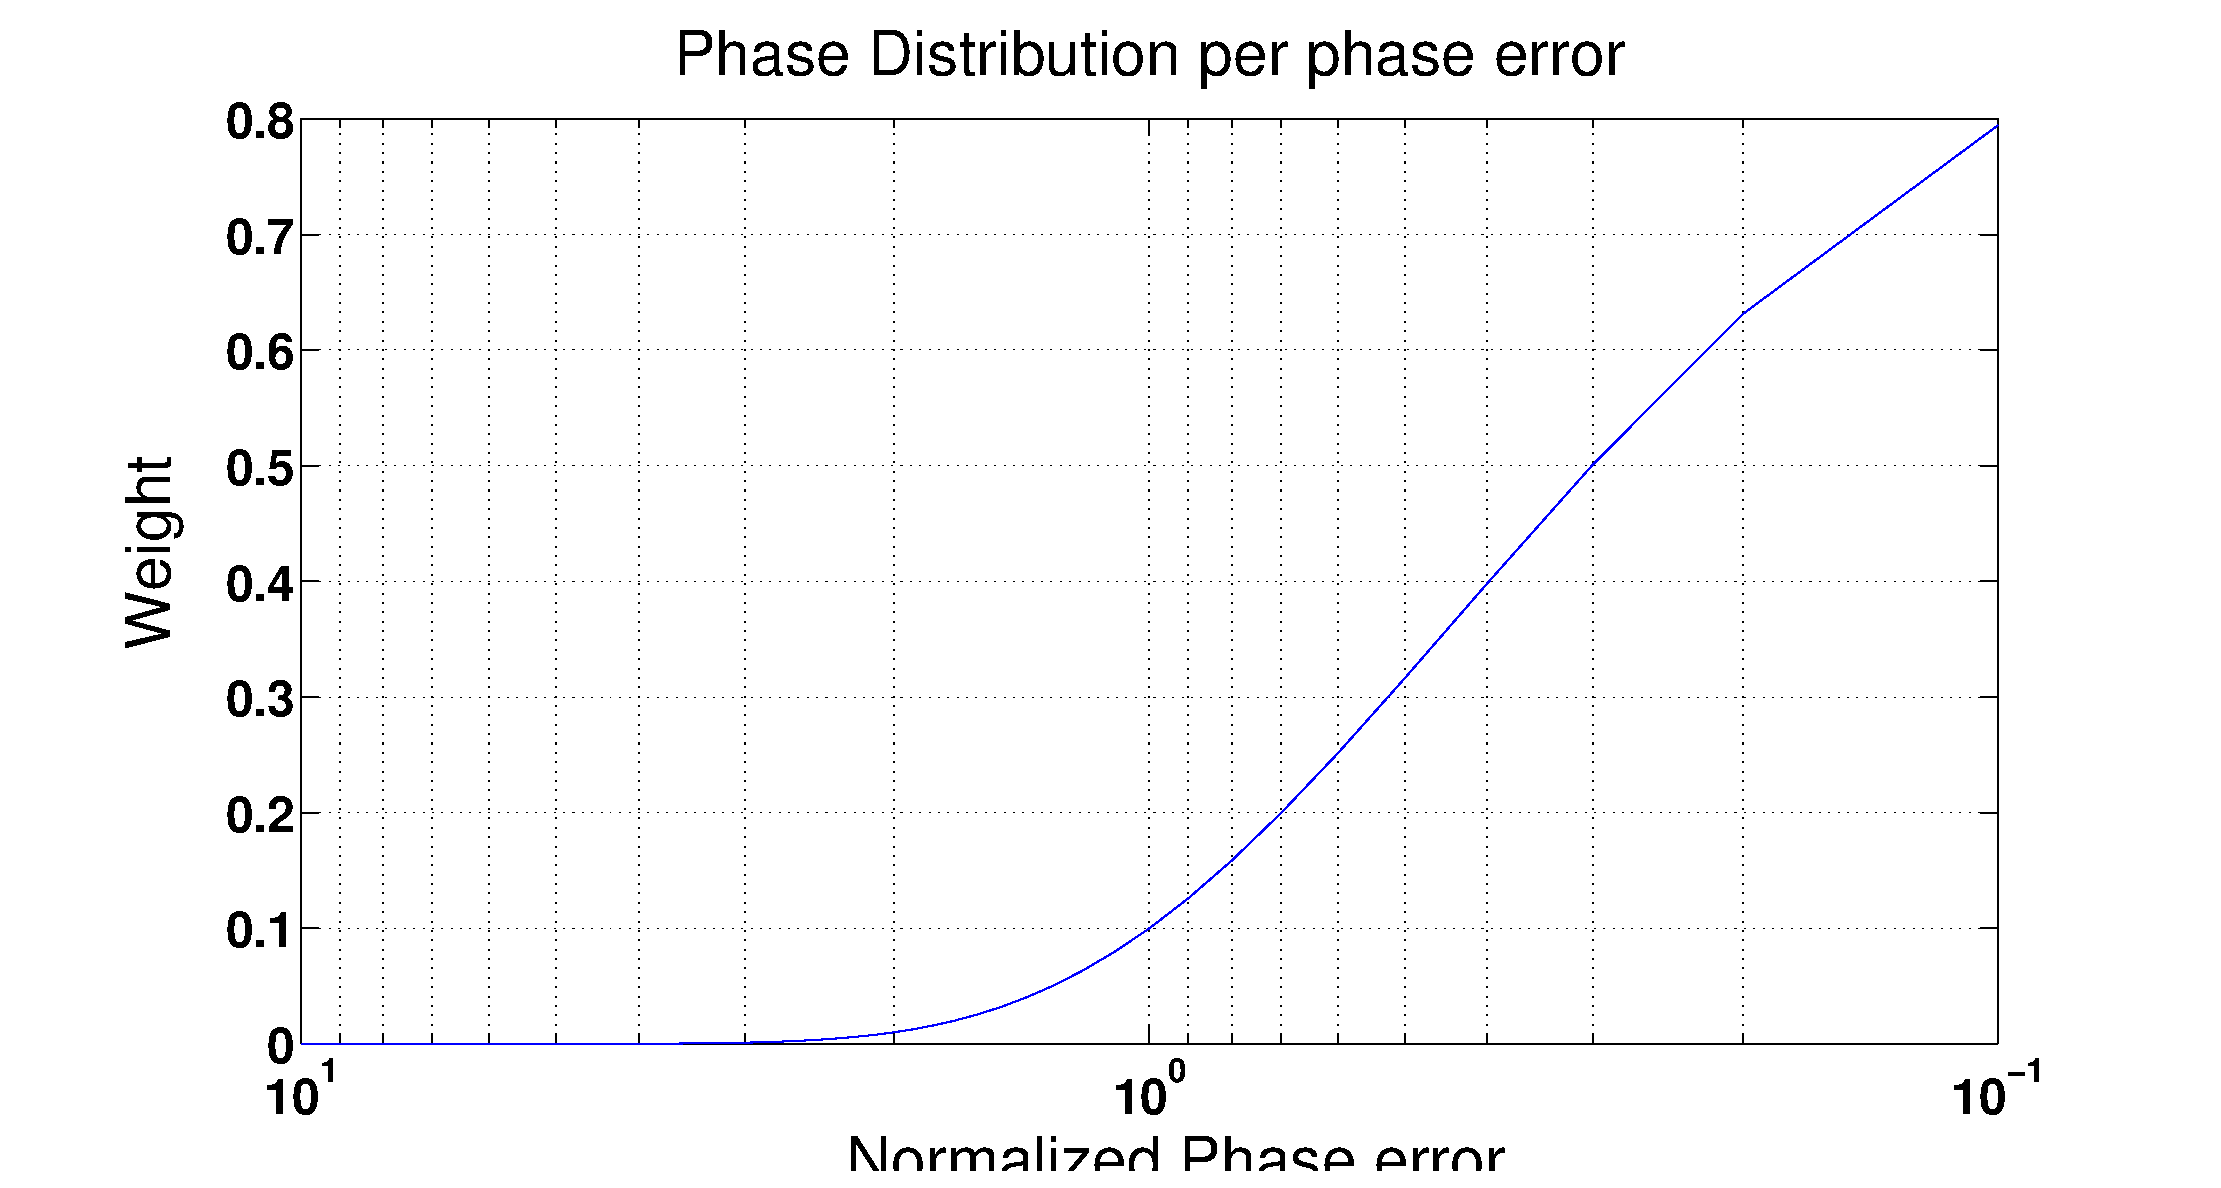
\includegraphics[width= 2.5in]{weight}
\caption{Weight factors for the phase error distribution}
\label{weight}
\end{figure}
The parameters $a$ and $b$ are selected using the initial conditions, $\delta_{ij}=0.1$ for $\Delta t_{ij}$ = $t_{guard}$ and $\delta_{ij}=1$ for $\Delta t_{ij}$ = 0.
\newline
As shown in Figure $\ref{weight}$, the closer the phase error is to zero, the
higher weight it is given. The assignment of high
values to the small phase errors will decrease the time it takes to
synchronize  this node with the network.
\newline
In the assignment of the weight factor, there is another issue to be
considered. If all the phase errors are in the lower region, this
corresponds to the fact that the node is a newly joining node to a
well-established and synchronized network.  In order to incorporate the
effect of the distribution of the phase errors, another step is introduced in the calculation of the weight factors so
that the node will adjust its wake-up time towards the more
stabilized network. \newline
The weight factor is
\[w_{ij} = \left\{
\begin{array}{l l}
  1 - \delta_{ij},& \quad \mbox{if $mean(\delta_{ij}$) $<$ 0.5}\\
 \delta_{ij}, & \quad \mbox{if $mean(\delta_{ij}$) $>$ 0.5}\\ \end{array} \right. \]
where $m$ is the mean function.
Hence, the weight moves towards the large phase errors if the node is a new-comer that wants to join the "already established"
network.
\newline As explained earlier, WM is a two step process in which the first one describes how the node has drifted away from its neighbors
whereas the second one describes how the node is positioned in the network topology which surrounds it.
\newline
Using the WM approach, a series of measurements will be used to estimate the next wake-up time of the node, giving less value/emphasis to the nodes which are out of reach from the neighboring nodes.
\subsubsection{\textbf{Non Linear Least Squares - Interference
elimination}}
\textbf{Non-Linear Least Squares} \newline
\begin{figure}[b]
\centering
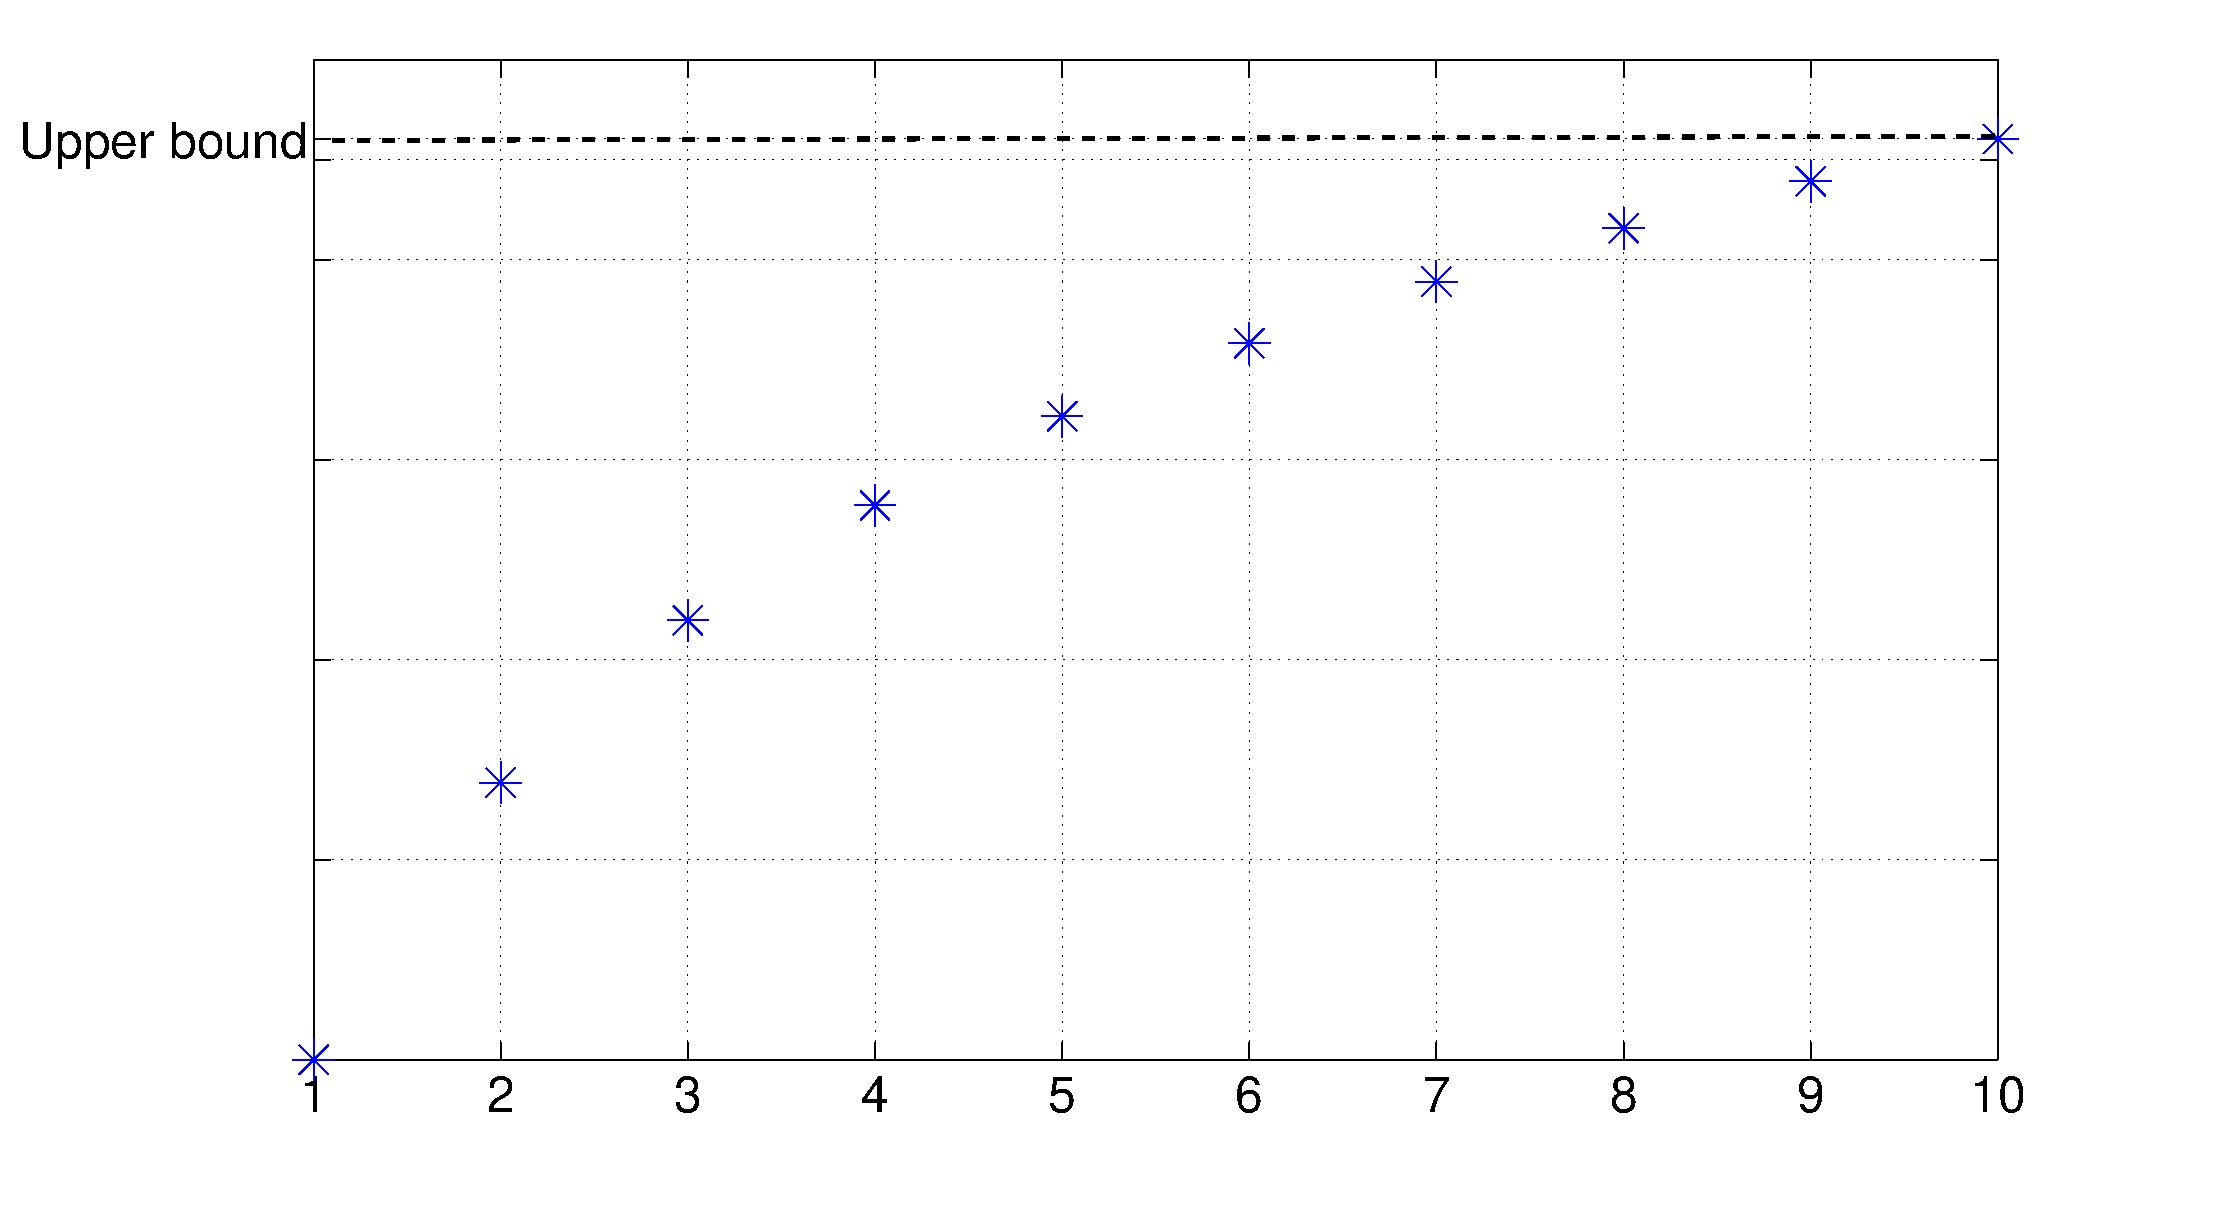
\includegraphics[width=2.5in]{curvefit}
\caption{Curve fitting using logarithmic function} \label{curvefit}
\end{figure}
Non Linear Least Squares (NLLS) curve fitting  is a mathematical procedure for
finding the best fitting curve to a given set of points by
minimizing the sum of the squares of the offsets ("the residuals")
of the points from the curve. \newline
In order to meet the demand of adjusting the time offset and stabilize the network, the logarithmic curve is chosen. A logarithmic function can be used to represent the distribution of the offsets in the neighborhood,
\begin{equation}
 f(x_i,\beta)= \beta _1 + \beta_2log(x_i),
\end{equation}
where $\beta_1$ and $\beta_2$ are the parameters to be estimated.\newline
Normalized phase error values tend to be small and follow a curve in such away that the maximum value of the phase error should not be greater than the threshold value that was intended to be, the synchronization error. See Figure $\ref{curvefit}$.
\newline
Using a set of $n$ data points(corresponding to $n$ neighbors) which are ($x_1$, $y_1$),
($x_2$, $y_2$),$\dots$,($x_n$, $y_n$), and a curve (model function)
$y= f(x, \beta)$, that in addition to the variable $x$ can be used to calculate the offset.
\newline
It is desired to find the vector $\beta$ of parameters $(\beta_1, \beta_2)$ such that the curve fits best the given data in the least squares, that is, the sum of squares
\begin{equation}
    S=\sum_{i=1}^{m}r_i^2 ,
\end{equation}
is minimized, where the residuals $r_i$ are given by
\begin{equation}
    r_i = y_i - f(x_i,\beta),
\end{equation}
for i=1,2,$\dots$, $n$.
\newline
The minimum value of $S$ occurs when the gradient is zero. Hence, there are gradient equations to be solved:
\begin{equation}
    \frac{\partial S}{\partial \beta_j}=2\sum_i r_i\frac{\partial r_i}{\partial \beta_j}=0 \ (j=1,2).
\end{equation}
In a non-linear system, the derivatives $\frac{\partial r_i}{\partial \beta_j}$ are functions of both the independent
variable and the parameters. These gradient equations do not have a
closed solution. Instead, initial values must be chosen for the
parameters. Then, the parameters are refined iteratively, that is,
the values are obtained by successive approximation,
\begin{equation}
    \beta_j^{k+1}=\beta^k_j+\Delta \beta_j.
\end{equation}
Here, $k$ is an iteration number and the vector of increments, $\Delta \beta_j$, is known as the shift vector. At each iteration,
the model is linearized by approximation to a first-order Taylor series expansion about $\beta^k$.
\begin{equation}
    f(x_i,\beta)\approx f(x_i,\beta^k) +\sum_j \frac{\partial f(x_i, \beta^k)}{\partial \beta_j} \left(\beta^k_j -\beta_j \right)
\end{equation}
\begin{equation}
 f(x_i,\beta) =f(x_i, \beta^k)+\sum_j J_{ij} \Delta\beta_j.
\end{equation}
The Jacobian, $J$, is a function of constants, the independent
variable and the parameters, so it changes from one iteration to the
next. Thus, in terms of the linearized model,
\begin{equation}
\frac{\partial r_i}{\partial \beta_j}=-J_{ij}
\end{equation}
and the residuals are given by
\begin{equation}
    r_i=\Delta y_i- \sum_{j=1}^{j=2} J_{ij}\Delta\beta_j,
\end{equation}
where
\begin{equation}
 \Delta y_i=y_i- f(x_i, \beta^k).
\end{equation}
Substituting these expressions into the gradient equations and
equating to $0$, a matrix notation can be found
\begin{equation}
    \left(J^TJ\right)\Delta  \beta=J^T\Delta y
\end{equation}
When the observations are not equally reliable, as in case of WSNs
which are being studied, a weighted sum of squares may be minimized
using the weights (Figure $\ref{weight}$),
\begin{equation}
    S=\sum_{i=1}^{i=n}W_{ii}r_i^2.
\end{equation}
The normal equations are then
\begin{equation}
    \left(J^TWJ\right)\Delta  \beta=J^TW\Delta y.
\end{equation}
\textbf{Model Design}\newline
As the algorithm is decentralized, the next wake-up time of the node depends on the current offset that it has with the other nodes. The distribution of the phase error is the crucial factor in deciding the type of curve to fit in. The phase errors shows how many time units that the neighbor node is out of touch with the node in focus. The larger the phase error is, the more out-of-sync the node is.\newline
The set of data are the measured phase errors of the node and the parameters $\beta_1$ and $\beta_2$ are estimated using a least squares approximation for the function
\begin{equation}
 f(x_i,\beta)= \beta _1 + \beta_2log(x_i),
\end{equation}
The initial values of the parameters $\beta_1$ and $\beta_2$ is estimated taking into account
the state of the network to be. \newline
As each measurement arrives from the neighbors, the parameters are calculated in such a way that the measurement error from a pre-determined offset value is reduced. This ensures that the offset to be added in the next wake-up time doesn't diverge in a large amount from the predicted value.
\subsubsection{\textbf{Discrete time Kalman Filter for synchronization}}
\textbf{Discrete time Kalman Filter} \newline
The Kalman Filter estimates a process by using a form of feedback
control: the filter estimates the process state at some time and
then obtains feedback in the form of (noisy) measurements. As such,
the equations for the Kalman filter fall into two groups: time
update equations and measurement update equations. The time update
equations are responsible for projecting forward (in time) the
current state and error covariance estimates to obtain the a priori
estimates for the next time step.
\newline
The Kalman filter addresses the general problem of trying to
estimate the state $x$ of a discrete-time controlled process that is
governed by the linear stochastic difference equation
\begin{equation}
 x_k = Hx_{k-1} + Bu_k + w_{k-1} ,
\end{equation}
with a measurement $z$ that is
\begin{equation}
 z_k = Hx_k + v_k.
\end{equation}
The random variables $w_k$ and $v_k$ represent the process and
measurement noise (respectively). They are assumed to be
independent (of each other), white, and with normal probability
distributions
\begin{equation}
 p(w) \approx N(0,Q),
\end{equation}
\begin{equation}
 p(v) \approx N(0,R).
\end{equation}
With the initial estimates of $x_{k-1}$ and $P_{k-1}$
\begin{equation}
x_k = Hx_{k-1} + Bu_k
\end{equation}
\begin{equation}
P_k = HP_{k-1}H^T + Q.
\end{equation}
The measurement update equations are responsible for the feedbacks
i.e. for incorporating a new measurement into the a priori estimate
to obtain an improved a posteriori estimate.
\begin{equation}
K_k = P_kH^T(HP_kH^T + R)^{-1} \label{kalmangain}
\end{equation}
\begin{equation}
x_k = x_k + K_k(z_k - Hx_x)
\end{equation}
\begin{equation}
P_k = (I-K_kH)P_k
\end{equation}
The time update equations can also be thought of as predictor
equations, while the measurement update equations can be thought of
as corrector equations.
\newline
Hence, a priori and a posteriori estimate errors are defined as
\begin{equation}
e_k^- = x_k – \tilde x_k^- ,
\end{equation}
\begin{equation}
e_k =  x_k – \tilde x_k.
\end{equation}
The a priori estimate error covariance is then
\begin{equation}
P_k^- = E[ e_k^- e_k^{-T} ]
\end{equation}
and the a posteriori estimate error covariance is
\begin{equation}
P_k = E[e_k e_k^T]
\end{equation}
The update equation is
\begin{equation}
\tilde x_k = \tilde x_k + K(z_k-H\tilde x_k).
\label{updatekalman}
\end{equation}
The difference $z_k - H\tilde x_k$ in ($\ref{updatekalman}$) is called
the residual. The residual reflects the discrepancy between the
predicted measurement $H\tilde x_k$ and the actual measurement
$z_k$. A residual of zero means that the two are in complete
agreement. \newline
The matrix K in ($\ref{kalmangain}$) is
chosen to be the gain or blending factor that minimizes the
posteriori error covariance. Taking the derivative of the trace of
the result with respect to K, setting that result equal to zero, and
then solving for K,
\begin{equation}
K_k = P_kH^{T}(HP_kH^{T} + R)^{-1}
\end{equation}
\begin{equation}
K_k = \frac{P_kH^T}{HP_kH^T + R}. \label{gain}
\end{equation}
Looking at ($\ref{gain}$), it is seen that as the measurement error
covariance $R$ approaches zero, the gain K weights the residual more
heavily. Specifically,
\begin{equation}
\mathop {\lim }\limits_{R_k \to 0 } {K_k} = H^{-1}.
\end{equation}
On the other hand, as the a priori estimate error covariance $P_k$
approaches zero, the gain K weights the residual less heavily.
Specifically,
\begin{equation}
\mathop {\lim }\limits_{P_k \to 0 } {K_k} = 0.
\end{equation}
\textbf{Filter design} \newline
The transition matrix $H$ plays an important role in achieving
the proper synchronization. It indicates how fast/slow is the next wake up time should be compared
to it's previous value and/or neighbors. With the stable network where the nodes remain intact,
the wake-up time of the node is expected to be the same despite the
clock drift.
\newline
The initial estimates are selected from the previous firing time of the node.
Hence, the initial values of $x$ and $P$ are estimated from the previous values, one period earlier.
This ensures that the nodes are on the same track as the previous time, since the neighbors
remain the same with some exception of mobility and interference.
Hence, to tackle the dynamic nature of the WSN, the
new node joining the network should be synchronized with the already
established "status quo" of the network.
In the filter design, the covariance matrices $R$ and $Q$ have a significant
role in the overall implementation of the algorithm. $R$ represents how
 the measurments are valued to affect the result of the outcome and $Q$
sends a signal as to how the estimated value is weighed.
\subsection{\textbf{Reducing the guard time}}
As the perfromance of the algorithms increase, the guard time can also be reduced to conserve energy. This inturn
reduces the duty cycle.
\begin{figure}[b]
\centering
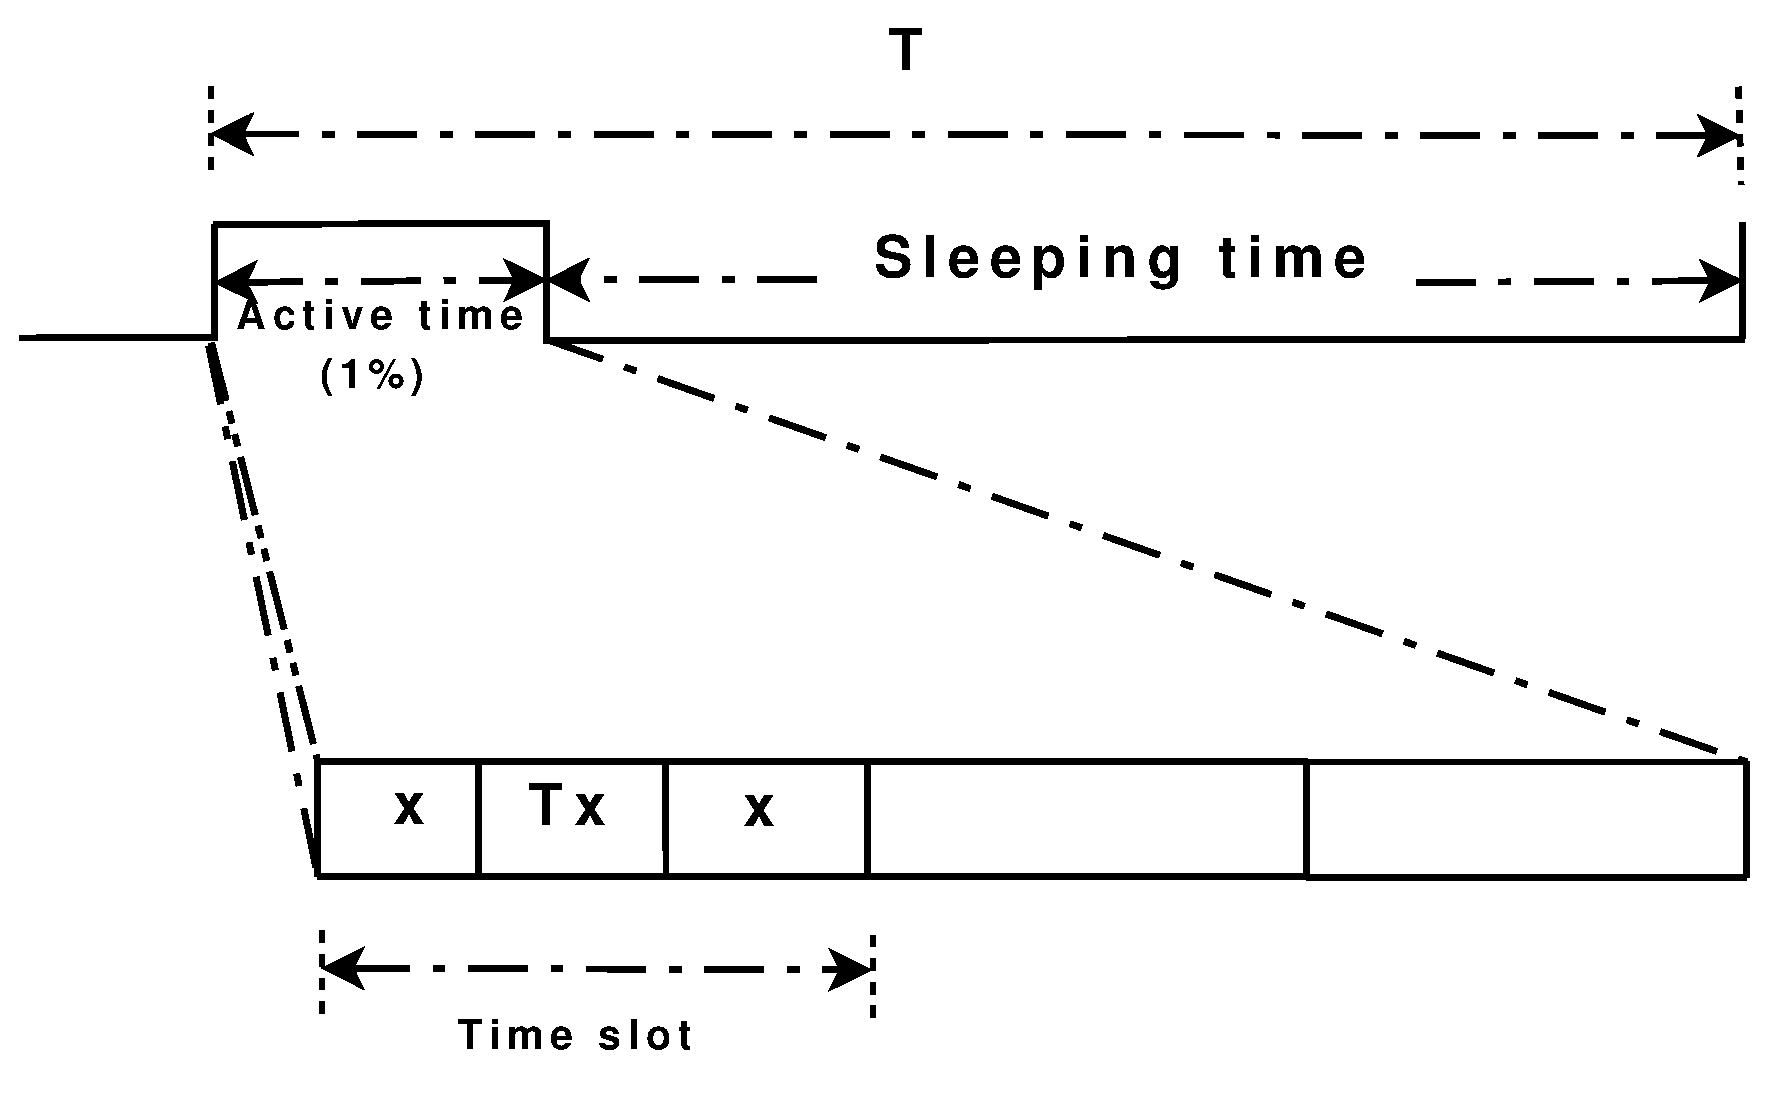
\includegraphics[width=2.5in]{guardtimesaving}
\caption{Guard time saving} \label{guardtimesaving}
\end{figure}
\newline Let $x$ denote the guard time when the median algorithm is
implemented (Figure $\ref{guardtimesaving}$). Thus, the slot
duration will be
\begin{equation}
T_{slot}=2x + T_x ,
\label{slot}
\end{equation}
where $T_x$ is the transmit time of the node. \newline
With $N$ slots, the duty cycle is then
\begin{equation}
D = \frac{NT_{slot}}{T}, \label{duty}
\end{equation}
where $T$ is the period of a time frame. \newline Substituting
($\ref{slot}$) in ($\ref{duty}$) equation, the duty cycle becomes
\begin{equation}
D= \frac{N(2x+T_{slot})}{T}.
\end{equation}
With the better performance achievement with the other algorithms,
the guard time can be reduced depending on the precision of the
algorithm. Let $\epsilon$ be the guard time reduction in clock
cycles. The new guard time will be $2x-\epsilon$.\newline The
new duty cycle becomes
\begin{equation}
D_n=\frac{(2(x-\epsilon)+T_x)N}{T}.
\end{equation}
Arranging the equation results in
\begin{equation}
D_n= \frac{(2x+T_x)N}{T} - \frac{(2\epsilon)N}{T}.
\end{equation}
Hence, with a performance increase in $\epsilon$ clk results in the
duty cycle reduction of
\begin{equation}
D - D_n = \frac{(2\epsilon)N}{T}.
\end{equation}
The decrease in the guard time of the slot is thus dependent on the
algorithm's performance ($\epsilon$) and the number of slots in the
frame. As the number of slots increases with a constant performance increase $\epsilon$, the energy conservation
also increases linearly.
\section{\textbf{Results and Discussion}}
\subsection{\textbf{Simulation setup}}
\noindent In the simulation, a Discrete Event Simulator (DES) is used. A DES will break down a simulation into discrete chunks. Every event will occur at some countable time moment and will be given in chronological order. The
advantage of this distinction is two-fold. First, simulations will
not be dependant on some real-time clock. Second, events can be
isolated to perform certain measurements.
\newline
One such DES is MiXiM$\footnote{MiXiM (Mixed Simulator) is a simulation framework for wireless and mobile networks using the OMNeT++ $\cite{omnet}$ simulation engine. It is a collaborative project between TU Berlin, TU Delft and Universitaet Paderborn.}$. It provides a component architecture for models. Components are programmed in C++, then assembled into larger components and models using a high-level language. Octave$\footnote{Octave is a free program for performing numerical computations which is mostly compatible with MATLAB. It is part of the GNU project.}$ is used for interpretation of the data from the network simulator.
\newline
The simulation is conducted 1000 times to counter the effect of randomness introduced in the
simulation.
\subsection{\textbf{Simulation Results}}
\begin{figure*}
\centerline{
\subfloat[Number of Nodes - 20]{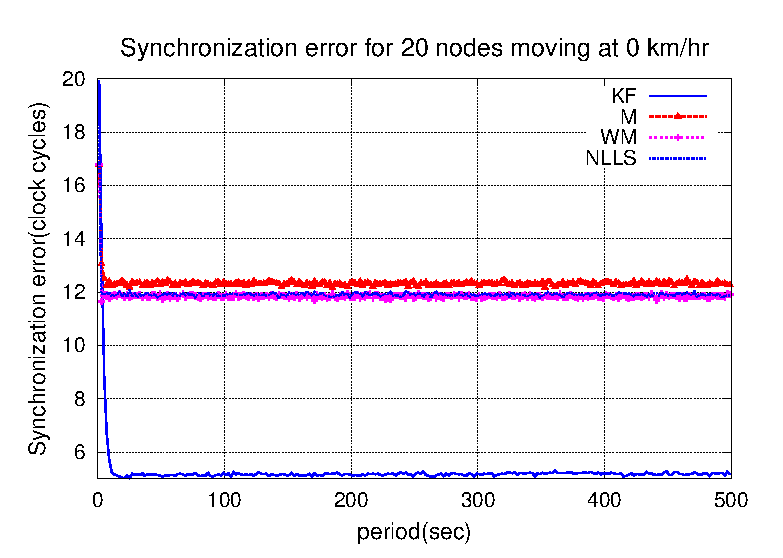
\includegraphics[width=2.5in]{16output-s0}
\label{16output0}}
\hfil
\subfloat[Number of Nodes - 50]{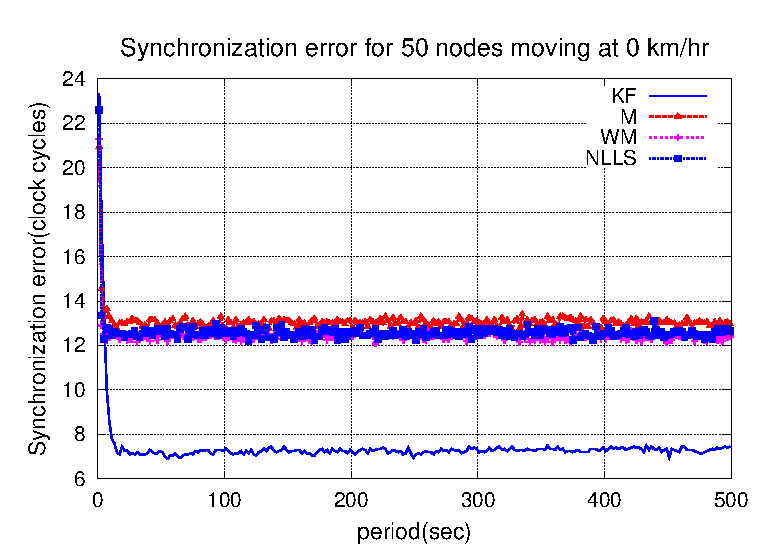
\includegraphics[width=2.5in]{50output-s0}
\label{50output0}}}
\caption{Simulation results for Static Nodes }
\label{static}
\end{figure*}
The nodes are deployed uniformly across the field. The neighborhood is limited
to 10 nodes. The start up time of the
nodes is random, Gaussian distributed variable, $t_{io}$. The
synchronization error is the difference between the wake-up time of the nodes in the
neighborhood.
\subsubsection{\textbf{Case I}} In the first set of simulation, the
synchronization error is simulated for the nodes which are static,
hence no effect of mobility. The number of nodes is taken to be $20$
and $50$ in the set of simulations.
\newline
Figure $\ref{16output0}$ shows the synchronization error for $20$ nodes operating in a static environment. KF has the lowest synchronization error, at an avergage of $4clk$. NLLS and WM perform similarly with Median at average of
$12clk$. \newline
Figure $\ref{50output0}$ is the result of a simulation for $50$ nodes. The synchronization error in general increases as the number of nodes increases the number of neighbors, resulting in more data for the synchronization layer. Comparing the individual algorithms, KF has over $7clk$ performance improvement than the Median whereas NLLS and WM have a better performance ($1clk$) than the Median.
\subsubsection{\textbf{Case II}}
\begin{figure*}
\centerline{
\subfloat[Speed - 6km/hr]{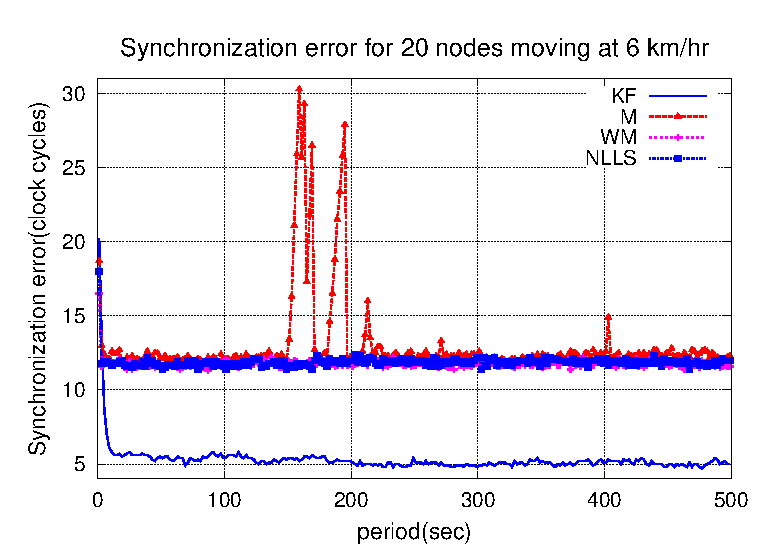
\includegraphics[width=2.5in]{16output-s6}
\label{16output6}} \hfil \subfloat[Speed -
20km/hr]{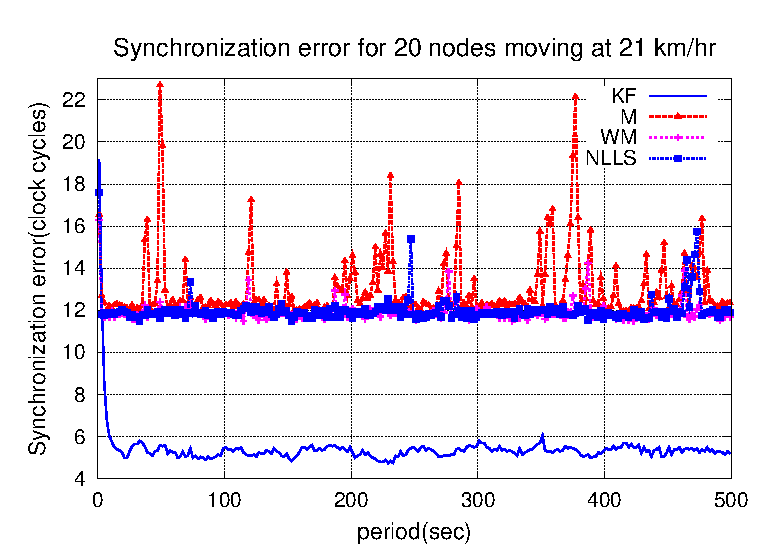
\includegraphics[width=2.5in]{16output-s20}
\label{16output20}}} \caption{Simulation results for 20 Nodes}
\label{16output}
\end{figure*}
In second set of simulations, the mobility of the nodes is taken
into account. Here, the number of the nodes is taken to be $20$. The
simulations are conducted for different speeds, at $6km/hr$ and
$20km/hr$. Chosen speeds emulate the speed of a walking man and an
average speed of a slowly moving vehicle. \newline Figure
$\ref{16output6}$ shows 20 nodes with a constant speed of $6km/hr$
random mobility. As the results shows, WM and NLLS perform better
the synchronization of the frame, $1 clk$ each. KF outperforms all
the best, with $8 clk$ from the Median algorithm. \newline The
simulation is also conducted with a speed of $20km/hr$, having
similar results(Figure $\ref{16output20}$). With the increase in the
speed of the nodes, the precision of the algorithms improves. KF,
with an average of of $10 clk$ performs the best, whereas WM and
NLLS perform well too compared with the median, $1 clk$ and $1 clk$
respectively. \newline
The relative comparison of the algorithms performance improvement with the Median is shown in Figure $\ref{16relerror}$. WM
and NLLS perform, on average, $8-10\%$ better than Median. The best
performer, KF, has on average $60\%$ better performance than the
Median one.
\begin{figure}
\centering 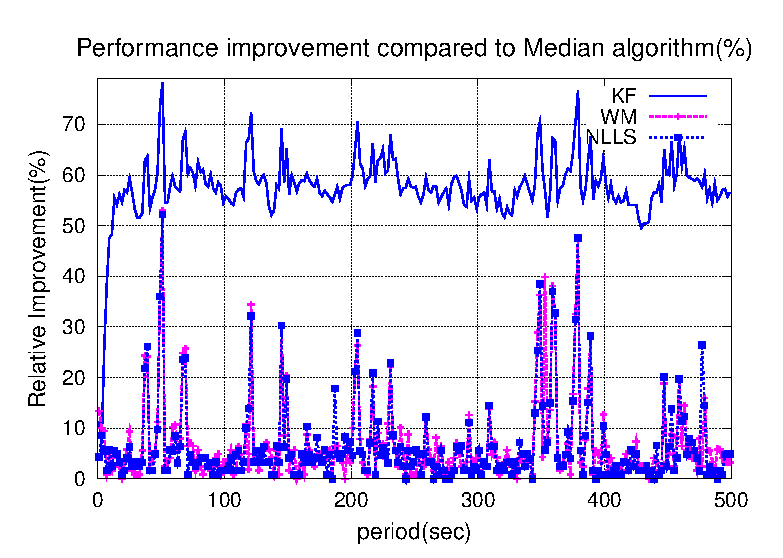
\includegraphics[width=2.5in]{16output-error}
\caption{Relative error of the algorithms w.r.t. Median}
\label{16relerror}
\end{figure}
\subsubsection{\textbf{Case III}}
\begin{figure*}
\centerline{ \subfloat[Speed -
6km/hr]{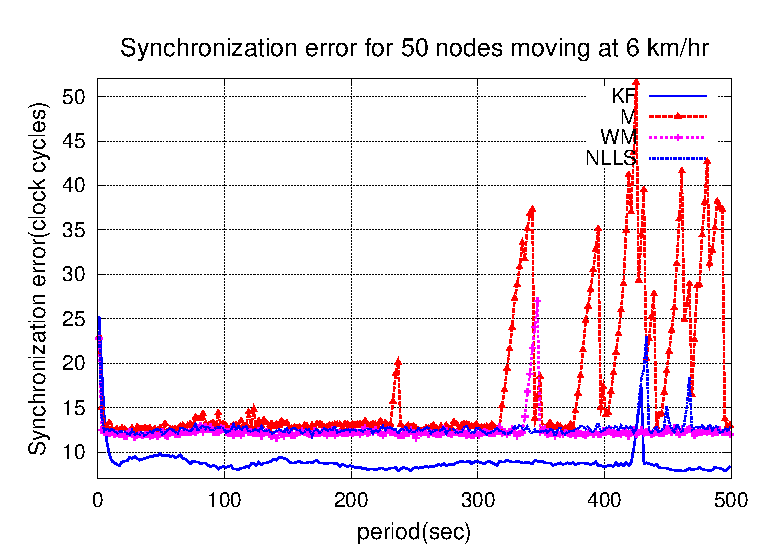
\includegraphics[width=2.5in]{50output-s6}
\label{50output6}} \hfil \subfloat[Speed -
20km/hr]{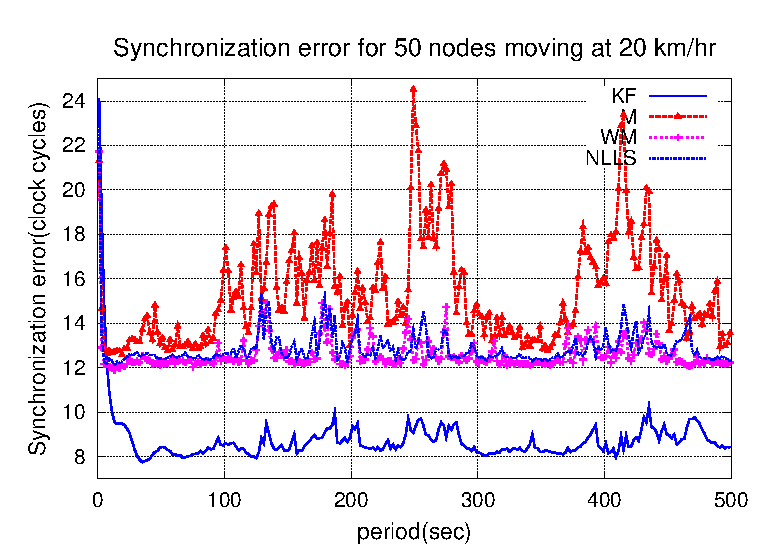
\includegraphics[width=2.5in]{50output-s20}
\label{50output20}}} \caption{Simulation results for 50 Nodes}
\label{50output}
\end{figure*}
In this set of simulations, the number of the nodes is increased to
$50$. With slowly moving nodes ($6km/hr$), the results are shown in
Figure $\ref{50output6}$. Large disruptions occur due to nodes
moving slowly in the surrounding (leave the network and join again
after some time), resulting in a larger drift with neighbors before
getting back to the network. \newline With a speed of $20km/hr$, the
simulation result is presented in Figure $\ref{50output20}$. With
this speed, the performance is better due to the faster moving
nodes, joining the networks at a faster rate. This helps in getting
synchronized with the nodes in a faster time, without drifting away
for a longer period of time(which is the case in the first set of
nodes with speed of $6km/hr$). Again, for the set of nodes with a
higher speed , a relative comparison is made to see the performance
of the nodes with the median algorithm.\newline The Median
algorithms is shown to perform the worst in this case. There are a
lot of disruptions in the network, making it more unstable whereas
the other algorithms adapt to the changes faster.\newline
Figure $\ref{50relerror}$ shows that KF performs the best
against Median algorithm, $45\%$. WM and NLLS perform well against
Median too, $5\%$ each. It has been shown that the median is
prone to error in case of high dynamics in the network.
\begin{figure}
\centering 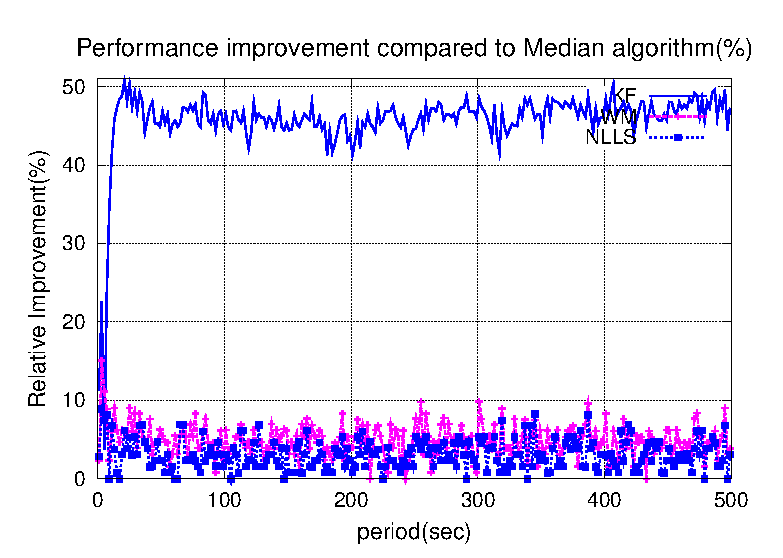
\includegraphics[width=2.5in]{50output-error}
\caption{Relative error of the algorithms w.r.t. Median}
\label{50relerror}
\end{figure}
In general, the Kalman filter has a better precision and convergence
speed than the rest whereas WM and NLLS has a better tolerance to a dynamic network.
\subsection{\textbf{Measurements concerning the energy consumption}}
\begin{figure}[b]
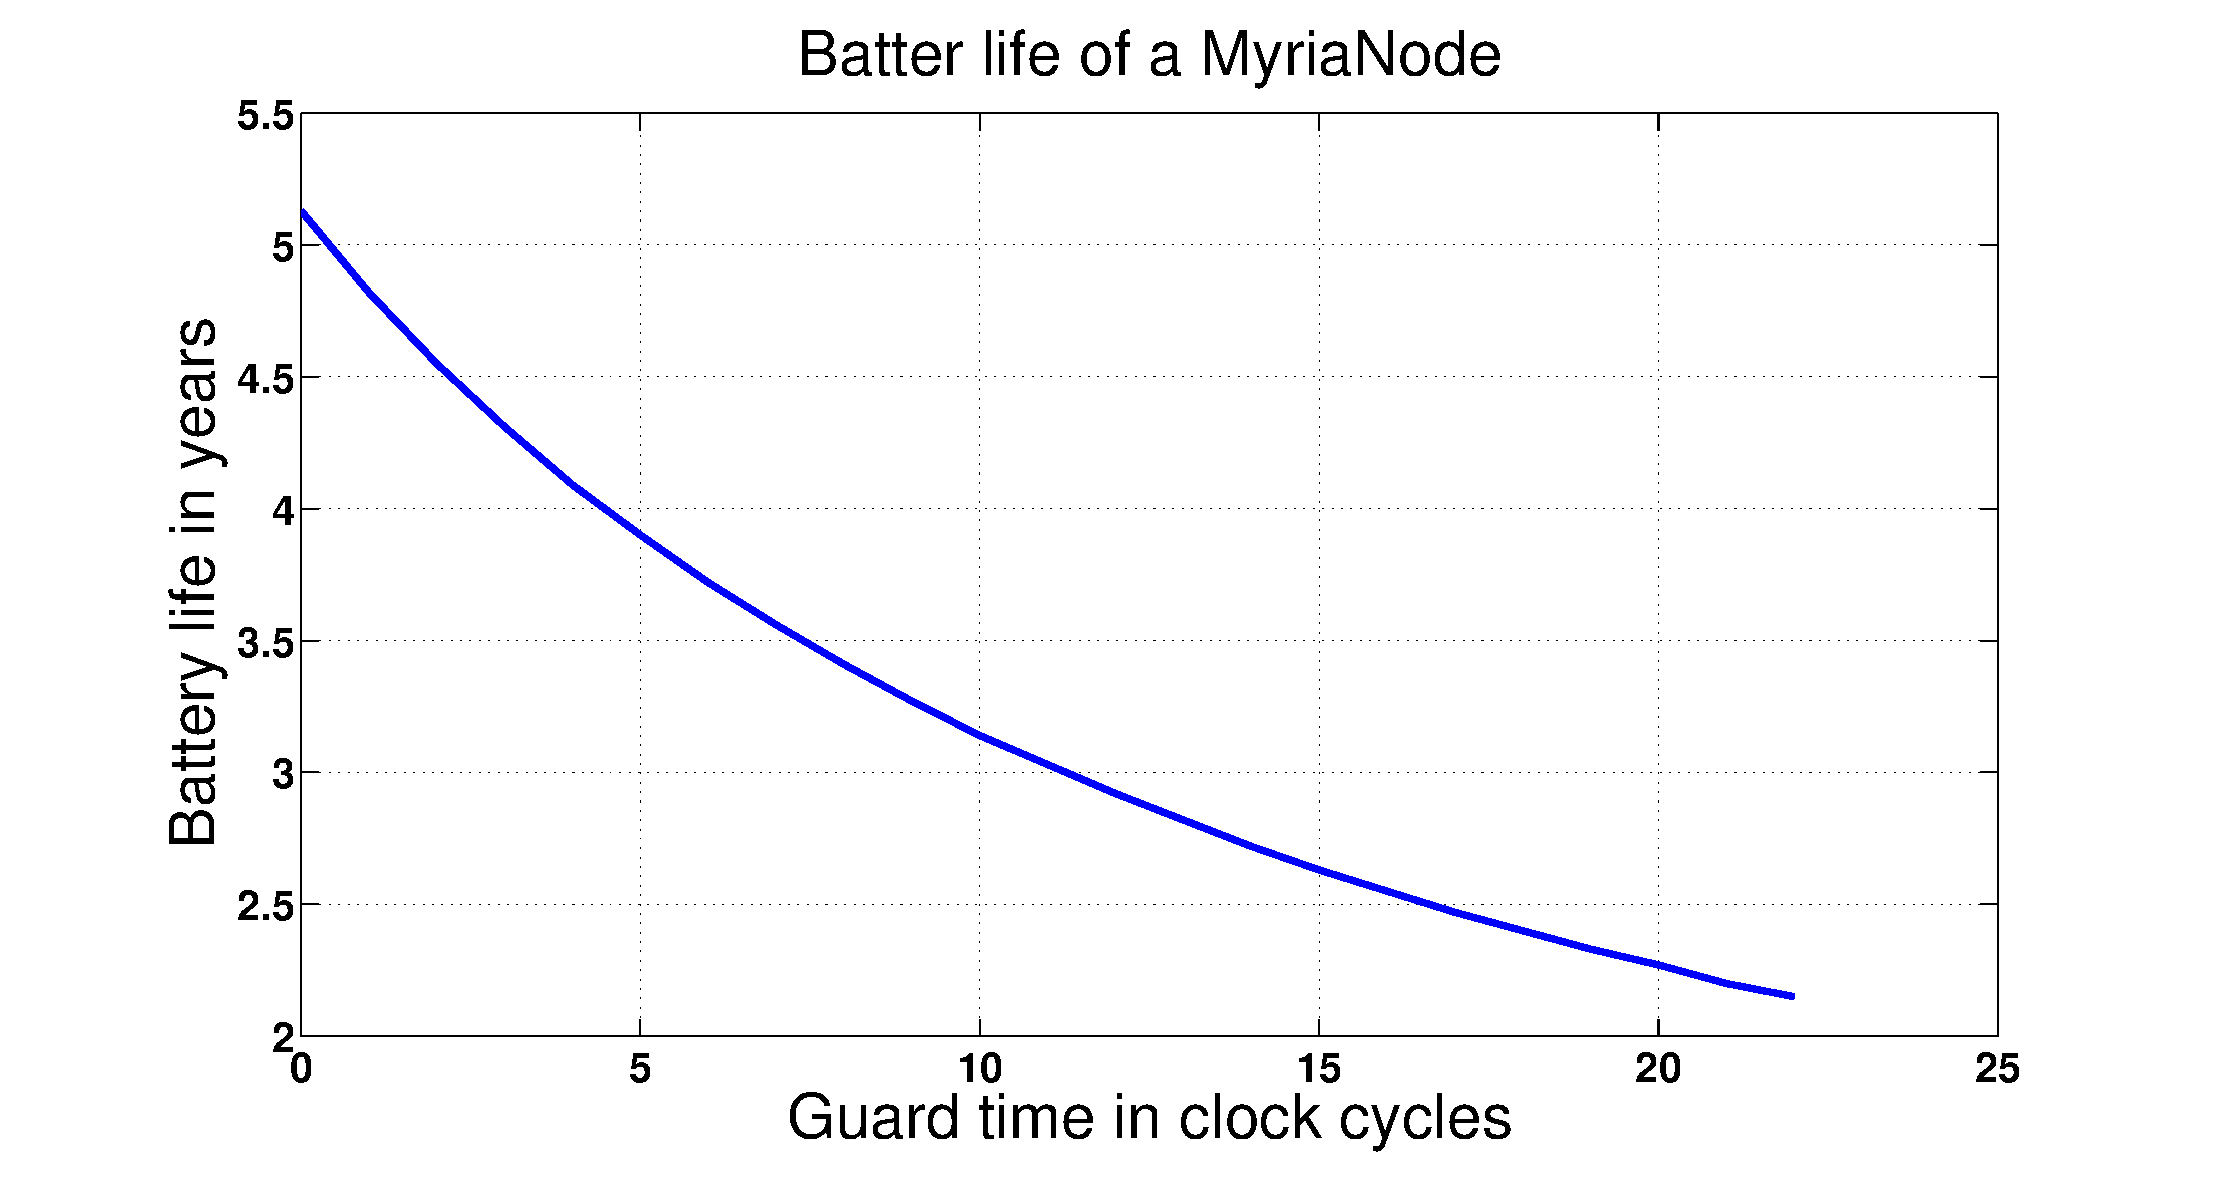
\includegraphics[width=0.5\textwidth]{guardsave}
\caption{The energy consumption of Guard time per RX slot}
\label{energyguard}
\end{figure}
As the results in the previous section shows, KF algorithm performs
well in all conditions, so do WM and NLLS. The downside in
implementing these algorithms, despite the performance gain that all
have against the Median is the energy consumption. As the algorithms
are going to be implemented on the sensor nodes, the energy
consumption is a priority in the study of embedded system algorithm
development. The algorithms are written in C and implemented on the
test nodes to see the effect that they are going to have on the
energy consumption of the nodes.
\begin{center}
    \begin{tabular}{ |p{2cm} | p{2.75cm} |}
    \hline
    Algorithm & Average Execution Time \\ \hline
    M &  65 $\mu$s \\ \hline
    NLLS & 82.5 $\mu$s \\ \hline
    WM &   90 $\mu$s \\ \hline
    KF &  150 $\mu$s  \\ \hline
    \end{tabular}
\label{tab}
\end{center}
The table shows the average execution time of the algorithms implemented on the MyriaNode. This doesn't show the
exact energy consumption of the algorithms but it can give us an
approximation on the relative comparison of the algorithms about the
energy consumption on the MyriaNode. As the table shows, the
consumption of WM is 5$\%$ higher than the median algorithms. This
is also true for NLLS and KF which consume 9$\%$ and 4 $\%$ higher
than the median algorithm respectively. \newline
In order to reduce the energy that is going to be spent on the algorithm with
a better performance, the guard time of the slot can be reduced, due
to a better performance showing by KF, WM and NLLS. The energy
consumption of the guard time is shown in Figure $\ref{energyguard}$.
\newline
With the performance gain obtained, the guard time of the slot
can be decreased, hereby decreasing the energy consumption of the
node in general. Hence, by decreasing the guard time in proportion with the
performance enhancement, energy for the demand of
the algorithm can be saved.
\section{\textbf{Conclusion and Recommendation}}
\noindent A decentralized frame synchronization of a TDMA-based WSN is achieved
using Weighted Measurements(WM), Non Linear Least Squares(NLLS) and
Kalman Filter(KF) methods. A simulation is conducted with different scenarios, especially
taking the effect of mobility. A comparison of the algorithms with the currently implemented Median algorithm
is conducted and the results are presented.
\newline
In a static environment, the KF performs the best whereas the WM and NLLS have shown a similar performance as the
Median. In terms of convergence time, all have shown a similar performance.
\newline
A $60\%$ improvement in the performance of the synchronization can
achieved on average using the Kalman Filter for dynamic WSN. A lower
improvement, $5\%$ and $4\%$ is obtained using WM and NLLS methods
for the synchronization of TDMA frames. Both WM and NLLS show a better tolerance
against Median in a dynamic network. KF estimation of
the optimal offset is the best with its iterative capability and
adaptive nature.\newline Median is shown to be still the best choice in a static environment with the current implementation,with less energy consumption and simplicity into consideration. But, for dynamic networks, the other algorithms perform better, in terms of
performance.
\newline But in the downside, the energy consumption of the algorithms is
greater than the Median algorithm's energy consumption as the algorithms are more complex computationally. Analysis is made and presented about the energy saving made by decreasing the guard time of the slot.
\newline  As suggestions for future work, a Software Defined Radio (SDR) for the inspection of the nodes' wake-up times, evaluation and enhancements on the algorithms, being implemented on the MyriaNodes, can be used. In addition, different software power minimization techniques can be applied to further reduce the power consumption of the algorithms' implementation, making it more energy-efficient for implementation.  As part of reducing the phase error between the clocks, compensating the frequency error using the available resource on the sensor nodes can be used. This can be achieved using the resources like the temperature sensor in the
microcontroller of the MyriaNode.
\section{\textbf{Acknowledgment}}This research is part of the MyriaNed$\footnote{MyriaNed is a project to create a large
functional network of 10,000 nodes with wireless communication for
research on protocols, power management, programming models, and
security.}$ Project and is conducted at Chess$\footnote{Chess is a SME company specialized in innovative
technical systems and business critical solutions. Chess creates and
develops sophisticated solutions and products for electronic
systems, transactions and electronic payments, Machine to Machine
(M2M) systems, sensor applications and digital multimedia. Chess is
located in Haarlem, the Netherlands.}$ B.V. The author would like to thank Frits van der Wateren from Chess Innovation Team for his continuous support, suggestions and advice during the project. Many thanks to dr.ir. Peter Smulders, prof.dr.ir. Erik Fledderus and prof.dr.ir. Peter Baltus from TU/e for their guidance.
\begin{thebibliography}{\textbf{References}}
\bibitem{2}J.Elson, L.Girod, D.Estrin. Fine-grained network time synchronization using reference broadcasts. Proceedings of the 5th Symposium on Operating Systems Design and Implementation ,2002.
\bibitem{3}Q.Yang, and et al. A Decentralized Slot Synchronization Algorithm for TDMA-Based Ad Hoc Networks.
\bibitem{5}NTP Public Services Project http://support.ntp.org/bin/view/Main/WebHome.
\bibitem{taxonomy}E.Anceaume and I.Puaut. A taxonomy of clock synchronization algorithms. IRISA Research Report No. PI1103, IRISA, 1997.
\bibitem{17}Q.Yang and J.Shi. An interference elimination method for decentralized slot synchronization in TDMA-based wireless ad hoc network.
\bibitem{pieter} P.Anemaet. Determining G-MAC potential with $\{$S,L,SCP$\}$-MAC. Masters thesis. Technische Universteit Delft. Delft. August 2008.
\bibitem{6}R.John. Introduction to Quartz Frequency Standards. Technical Report SLCET-TR-92-1, Army Research Laboratory, Electronics and Power Sources Directorate. October 1992.
%\bibitem{7}J.Elson and D.Estrin. Time Synchronization for Wireless Sensor Networks. In Proceedings of the 15th International Parallel and Distributed Processing Symposium. IEEE Computer Society, April 23-27. 2001.
%\bibitem{9}K.Romer. Time Synchronization in Ad Hoc Networks. In Proceedings of the Second ACM International Symposium on Mobile Ad Hoc Networking and Computing, Long Beach, California. 2001.
\bibitem{10}H.Karl and A.Willig. Protocols and Architectures for Wireless Sensor Networks.p3-6. Wiley. July 2006.
\bibitem{11}C.Cordeiro and D.Agrawal. Ad hoc and Sensor Networks Theory and applications. p.429-441. World Scientific Publishing. 2006.
\bibitem{1}F.Zhao and  L.Guibas. Wireless Sensor Networks: an Information Processing approach. p.107-108. Elsevier. 2004.
\bibitem{texas} S.Raje. Time synchronization of in Network-centric sensor networks. Master research. University of Texas, Arlington. Texas. August 2005.
\bibitem{correlation}A.Ebner, H.Rohling, M.Lott, and R.Halfmann. Decentralized Slot Synchronization in Highly Dynamic Ad Hoc Networks. Proc. WPMC '02, Honolulu, Hawaii, Oct. 2002.
\bibitem{14}S.PalChaudhuri and et al. Adaptive Clock Synchronization in Sensor Networks, Information Processing in Sensor Networks, April 2004.
%\bibitem{16}G.Werner-Allen and et al. Firefly-inspired sensor network synchronicity with realistic radio effects. Proceedings of the 3rd international conference on Embedded networked sensor systems, San Diego, California. November 2005.
\bibitem{18} $http://www.golledge.co.uk/pdf/products/xtl\_sm/cc7v.pdf$
\bibitem{19} $http://pdfserv.maxim-ic.com/en/an/AN58.pdf$.
\bibitem{omnet}$http://www.omnetpp.org$.
\bibitem{kalm}$http://www.cs.unc.edu/~welch/kalman/$.
\end{thebibliography}
\end{document}
\textbf{``Unnecessary synchronization wastes resources; insufficient synchronization leads to poor application performance.'' }
\newline
\textbf{``Stay and believe your instincts rather than going for the change''}.
\newline
\textbf{A man with a watch knows what time it is. A man with two watches is never sure. }\newline
